\documentclass{scrartcl}

    % included at the top of the generated TeX file

\usepackage{tgcursor}

\usepackage[utf8]{inputenc}

\KOMAoptions{parskip=half*}
\KOMAoptions{paper=a4,twoside=false}
\KOMAoptions{numbers=noendperiod}

\addtokomafont{disposition}{\rmfamily}
\setcounter{tocdepth}{\subsectiontocdepth}

    \usepackage[breakable]{tcolorbox}
    \usepackage{parskip} % Stop auto-indenting (to mimic markdown behaviour)
    

    % Basic figure setup, for now with no caption control since it's done
    % automatically by Pandoc (which extracts ![](path) syntax from Markdown).
    \usepackage{graphicx}
    % Maintain compatibility with old templates. Remove in nbconvert 6.0
    \let\Oldincludegraphics\includegraphics
    % Ensure that by default, figures have no caption (until we provide a
    % proper Figure object with a Caption API and a way to capture that
    % in the conversion process - todo).
    \usepackage{caption}
    \DeclareCaptionFormat{nocaption}{}
    \captionsetup{format=nocaption,aboveskip=0pt,belowskip=0pt}

    \usepackage{float}
    \floatplacement{figure}{H} % forces figures to be placed at the correct location
    \usepackage{xcolor} % Allow colors to be defined
    \usepackage{enumerate} % Needed for markdown enumerations to work
    \usepackage{geometry} % Used to adjust the document margins
    \usepackage{amsmath} % Equations
    \usepackage{amssymb} % Equations
    \usepackage{textcomp} % defines textquotesingle
    % Hack from http://tex.stackexchange.com/a/47451/13684:
    \AtBeginDocument{%
        \def\PYZsq{\textquotesingle}% Upright quotes in Pygmentized code
    }
    \usepackage{upquote} % Upright quotes for verbatim code
    \usepackage{eurosym} % defines \euro

    \usepackage{iftex}
    \ifPDFTeX
        \usepackage[T1]{fontenc}
        \IfFileExists{alphabeta.sty}{
              \usepackage{alphabeta}
          }{
              \usepackage[mathletters]{ucs}
              \usepackage[utf8]{inputenc}
          }
    \else
        \usepackage{fontspec}
        \usepackage{unicode-math}
    \fi

    \usepackage{fancyvrb} % verbatim replacement that allows latex
    \usepackage{grffile} % extends the file name processing of package graphics 
                         % to support a larger range
    \makeatletter % fix for old versions of grffile with XeLaTeX
    \@ifpackagelater{grffile}{2019/11/01}
    {
      % Do nothing on new versions
    }
    {
      \def\Gread@@xetex#1{%
        \IfFileExists{"\Gin@base".bb}%
        {\Gread@eps{\Gin@base.bb}}%
        {\Gread@@xetex@aux#1}%
      }
    }
    \makeatother
    \usepackage[Export]{adjustbox} % Used to constrain images to a maximum size
    \adjustboxset{max size={0.9\linewidth}{0.9\paperheight}}

    % The hyperref package gives us a pdf with properly built
    % internal navigation ('pdf bookmarks' for the table of contents,
    % internal cross-reference links, web links for URLs, etc.)
    \usepackage{hyperref}
    % The default LaTeX title has an obnoxious amount of whitespace. By default,
    % titling removes some of it. It also provides customization options.
    \usepackage{titling}
    \usepackage{longtable} % longtable support required by pandoc >1.10
    \usepackage{booktabs}  % table support for pandoc > 1.12.2
    \usepackage{array}     % table support for pandoc >= 2.11.3
    \usepackage{calc}      % table minipage width calculation for pandoc >= 2.11.1
    \usepackage[inline]{enumitem} % IRkernel/repr support (it uses the enumerate* environment)
    \usepackage[normalem]{ulem} % ulem is needed to support strikethroughs (\sout)
                                % normalem makes italics be italics, not underlines
    \usepackage{mathrsfs}
    

    
    % Colors for the hyperref package
    \definecolor{urlcolor}{rgb}{0,.145,.698}
    \definecolor{linkcolor}{rgb}{.71,0.21,0.01}
    \definecolor{citecolor}{rgb}{.12,.54,.11}

    % ANSI colors
    \definecolor{ansi-black}{HTML}{3E424D}
    \definecolor{ansi-black-intense}{HTML}{282C36}
    \definecolor{ansi-red}{HTML}{E75C58}
    \definecolor{ansi-red-intense}{HTML}{B22B31}
    \definecolor{ansi-green}{HTML}{00A250}
    \definecolor{ansi-green-intense}{HTML}{007427}
    \definecolor{ansi-yellow}{HTML}{DDB62B}
    \definecolor{ansi-yellow-intense}{HTML}{B27D12}
    \definecolor{ansi-blue}{HTML}{208FFB}
    \definecolor{ansi-blue-intense}{HTML}{0065CA}
    \definecolor{ansi-magenta}{HTML}{D160C4}
    \definecolor{ansi-magenta-intense}{HTML}{A03196}
    \definecolor{ansi-cyan}{HTML}{60C6C8}
    \definecolor{ansi-cyan-intense}{HTML}{258F8F}
    \definecolor{ansi-white}{HTML}{C5C1B4}
    \definecolor{ansi-white-intense}{HTML}{A1A6B2}
    \definecolor{ansi-default-inverse-fg}{HTML}{FFFFFF}
    \definecolor{ansi-default-inverse-bg}{HTML}{000000}

    % common color for the border for error outputs.
    \definecolor{outerrorbackground}{HTML}{FFDFDF}

    % commands and environments needed by pandoc snippets
    % extracted from the output of `pandoc -s`
    \providecommand{\tightlist}{%
      \setlength{\itemsep}{0pt}\setlength{\parskip}{0pt}}
    \DefineVerbatimEnvironment{Highlighting}{Verbatim}{commandchars=\\\{\}}
    % Add ',fontsize=\small' for more characters per line
    \newenvironment{Shaded}{}{}
    \newcommand{\KeywordTok}[1]{\textcolor[rgb]{0.00,0.44,0.13}{\textbf{{#1}}}}
    \newcommand{\DataTypeTok}[1]{\textcolor[rgb]{0.56,0.13,0.00}{{#1}}}
    \newcommand{\DecValTok}[1]{\textcolor[rgb]{0.25,0.63,0.44}{{#1}}}
    \newcommand{\BaseNTok}[1]{\textcolor[rgb]{0.25,0.63,0.44}{{#1}}}
    \newcommand{\FloatTok}[1]{\textcolor[rgb]{0.25,0.63,0.44}{{#1}}}
    \newcommand{\CharTok}[1]{\textcolor[rgb]{0.25,0.44,0.63}{{#1}}}
    \newcommand{\StringTok}[1]{\textcolor[rgb]{0.25,0.44,0.63}{{#1}}}
    \newcommand{\CommentTok}[1]{\textcolor[rgb]{0.38,0.63,0.69}{\textit{{#1}}}}
    \newcommand{\OtherTok}[1]{\textcolor[rgb]{0.00,0.44,0.13}{{#1}}}
    \newcommand{\AlertTok}[1]{\textcolor[rgb]{1.00,0.00,0.00}{\textbf{{#1}}}}
    \newcommand{\FunctionTok}[1]{\textcolor[rgb]{0.02,0.16,0.49}{{#1}}}
    \newcommand{\RegionMarkerTok}[1]{{#1}}
    \newcommand{\ErrorTok}[1]{\textcolor[rgb]{1.00,0.00,0.00}{\textbf{{#1}}}}
    \newcommand{\NormalTok}[1]{{#1}}
    
    % Additional commands for more recent versions of Pandoc
    \newcommand{\ConstantTok}[1]{\textcolor[rgb]{0.53,0.00,0.00}{{#1}}}
    \newcommand{\SpecialCharTok}[1]{\textcolor[rgb]{0.25,0.44,0.63}{{#1}}}
    \newcommand{\VerbatimStringTok}[1]{\textcolor[rgb]{0.25,0.44,0.63}{{#1}}}
    \newcommand{\SpecialStringTok}[1]{\textcolor[rgb]{0.73,0.40,0.53}{{#1}}}
    \newcommand{\ImportTok}[1]{{#1}}
    \newcommand{\DocumentationTok}[1]{\textcolor[rgb]{0.73,0.13,0.13}{\textit{{#1}}}}
    \newcommand{\AnnotationTok}[1]{\textcolor[rgb]{0.38,0.63,0.69}{\textbf{\textit{{#1}}}}}
    \newcommand{\CommentVarTok}[1]{\textcolor[rgb]{0.38,0.63,0.69}{\textbf{\textit{{#1}}}}}
    \newcommand{\VariableTok}[1]{\textcolor[rgb]{0.10,0.09,0.49}{{#1}}}
    \newcommand{\ControlFlowTok}[1]{\textcolor[rgb]{0.00,0.44,0.13}{\textbf{{#1}}}}
    \newcommand{\OperatorTok}[1]{\textcolor[rgb]{0.40,0.40,0.40}{{#1}}}
    \newcommand{\BuiltInTok}[1]{{#1}}
    \newcommand{\ExtensionTok}[1]{{#1}}
    \newcommand{\PreprocessorTok}[1]{\textcolor[rgb]{0.74,0.48,0.00}{{#1}}}
    \newcommand{\AttributeTok}[1]{\textcolor[rgb]{0.49,0.56,0.16}{{#1}}}
    \newcommand{\InformationTok}[1]{\textcolor[rgb]{0.38,0.63,0.69}{\textbf{\textit{{#1}}}}}
    \newcommand{\WarningTok}[1]{\textcolor[rgb]{0.38,0.63,0.69}{\textbf{\textit{{#1}}}}}
    
    
    % Define a nice break command that doesn't care if a line doesn't already
    % exist.
    \def\br{\hspace*{\fill} \\* }
    % Math Jax compatibility definitions
    \def\gt{>}
    \def\lt{<}
    \let\Oldtex\TeX
    \let\Oldlatex\LaTeX
    \renewcommand{\TeX}{\textrm{\Oldtex}}
    \renewcommand{\LaTeX}{\textrm{\Oldlatex}}
    % Document parameters
    % Document title
    \newcommand*{\mytitle}{Unit 7: Random number generation and statistics}

    % Included at the bottom of the preamble

\usepackage{microtype}


\title{\mytitle}
\author{Richard Foltyn}
\hypersetup{pdfauthor={Richard Foltyn}, pdftitle={\mytitle}}

% Remove horizontal rules in a very hackish way
\renewcommand{\rule}[2]{}

\RequirePackage{xspace}


\newcommand*{\eg}{e.g.\@\xspace}
\newcommand*{\Eg}{E.g.\@\xspace}
\newcommand*{\etc}{etc.\@\xspace}
\newcommand*{\ie}{i.e.\@\xspace}
\newcommand*{\vs}{vs.\@\xspace}
\newcommand*{\viz}{viz.\@\xspace}
\newcommand*{\US}{U.S.\@\xspace}

    
    
    
    
    
% Pygments definitions
\makeatletter
\def\PY@reset{\let\PY@it=\relax \let\PY@bf=\relax%
    \let\PY@ul=\relax \let\PY@tc=\relax%
    \let\PY@bc=\relax \let\PY@ff=\relax}
\def\PY@tok#1{\csname PY@tok@#1\endcsname}
\def\PY@toks#1+{\ifx\relax#1\empty\else%
    \PY@tok{#1}\expandafter\PY@toks\fi}
\def\PY@do#1{\PY@bc{\PY@tc{\PY@ul{%
    \PY@it{\PY@bf{\PY@ff{#1}}}}}}}
\def\PY#1#2{\PY@reset\PY@toks#1+\relax+\PY@do{#2}}

\@namedef{PY@tok@w}{\def\PY@tc##1{\textcolor[rgb]{0.73,0.73,0.73}{##1}}}
\@namedef{PY@tok@c}{\let\PY@it=\textit\def\PY@tc##1{\textcolor[rgb]{0.24,0.48,0.48}{##1}}}
\@namedef{PY@tok@cp}{\def\PY@tc##1{\textcolor[rgb]{0.61,0.40,0.00}{##1}}}
\@namedef{PY@tok@k}{\let\PY@bf=\textbf\def\PY@tc##1{\textcolor[rgb]{0.00,0.50,0.00}{##1}}}
\@namedef{PY@tok@kp}{\def\PY@tc##1{\textcolor[rgb]{0.00,0.50,0.00}{##1}}}
\@namedef{PY@tok@kt}{\def\PY@tc##1{\textcolor[rgb]{0.69,0.00,0.25}{##1}}}
\@namedef{PY@tok@o}{\def\PY@tc##1{\textcolor[rgb]{0.40,0.40,0.40}{##1}}}
\@namedef{PY@tok@ow}{\let\PY@bf=\textbf\def\PY@tc##1{\textcolor[rgb]{0.67,0.13,1.00}{##1}}}
\@namedef{PY@tok@nb}{\def\PY@tc##1{\textcolor[rgb]{0.00,0.50,0.00}{##1}}}
\@namedef{PY@tok@nf}{\def\PY@tc##1{\textcolor[rgb]{0.00,0.00,1.00}{##1}}}
\@namedef{PY@tok@nc}{\let\PY@bf=\textbf\def\PY@tc##1{\textcolor[rgb]{0.00,0.00,1.00}{##1}}}
\@namedef{PY@tok@nn}{\let\PY@bf=\textbf\def\PY@tc##1{\textcolor[rgb]{0.00,0.00,1.00}{##1}}}
\@namedef{PY@tok@ne}{\let\PY@bf=\textbf\def\PY@tc##1{\textcolor[rgb]{0.80,0.25,0.22}{##1}}}
\@namedef{PY@tok@nv}{\def\PY@tc##1{\textcolor[rgb]{0.10,0.09,0.49}{##1}}}
\@namedef{PY@tok@no}{\def\PY@tc##1{\textcolor[rgb]{0.53,0.00,0.00}{##1}}}
\@namedef{PY@tok@nl}{\def\PY@tc##1{\textcolor[rgb]{0.46,0.46,0.00}{##1}}}
\@namedef{PY@tok@ni}{\let\PY@bf=\textbf\def\PY@tc##1{\textcolor[rgb]{0.44,0.44,0.44}{##1}}}
\@namedef{PY@tok@na}{\def\PY@tc##1{\textcolor[rgb]{0.41,0.47,0.13}{##1}}}
\@namedef{PY@tok@nt}{\let\PY@bf=\textbf\def\PY@tc##1{\textcolor[rgb]{0.00,0.50,0.00}{##1}}}
\@namedef{PY@tok@nd}{\def\PY@tc##1{\textcolor[rgb]{0.67,0.13,1.00}{##1}}}
\@namedef{PY@tok@s}{\def\PY@tc##1{\textcolor[rgb]{0.73,0.13,0.13}{##1}}}
\@namedef{PY@tok@sd}{\let\PY@it=\textit\def\PY@tc##1{\textcolor[rgb]{0.73,0.13,0.13}{##1}}}
\@namedef{PY@tok@si}{\let\PY@bf=\textbf\def\PY@tc##1{\textcolor[rgb]{0.64,0.35,0.47}{##1}}}
\@namedef{PY@tok@se}{\let\PY@bf=\textbf\def\PY@tc##1{\textcolor[rgb]{0.67,0.36,0.12}{##1}}}
\@namedef{PY@tok@sr}{\def\PY@tc##1{\textcolor[rgb]{0.64,0.35,0.47}{##1}}}
\@namedef{PY@tok@ss}{\def\PY@tc##1{\textcolor[rgb]{0.10,0.09,0.49}{##1}}}
\@namedef{PY@tok@sx}{\def\PY@tc##1{\textcolor[rgb]{0.00,0.50,0.00}{##1}}}
\@namedef{PY@tok@m}{\def\PY@tc##1{\textcolor[rgb]{0.40,0.40,0.40}{##1}}}
\@namedef{PY@tok@gh}{\let\PY@bf=\textbf\def\PY@tc##1{\textcolor[rgb]{0.00,0.00,0.50}{##1}}}
\@namedef{PY@tok@gu}{\let\PY@bf=\textbf\def\PY@tc##1{\textcolor[rgb]{0.50,0.00,0.50}{##1}}}
\@namedef{PY@tok@gd}{\def\PY@tc##1{\textcolor[rgb]{0.63,0.00,0.00}{##1}}}
\@namedef{PY@tok@gi}{\def\PY@tc##1{\textcolor[rgb]{0.00,0.52,0.00}{##1}}}
\@namedef{PY@tok@gr}{\def\PY@tc##1{\textcolor[rgb]{0.89,0.00,0.00}{##1}}}
\@namedef{PY@tok@ge}{\let\PY@it=\textit}
\@namedef{PY@tok@gs}{\let\PY@bf=\textbf}
\@namedef{PY@tok@gp}{\let\PY@bf=\textbf\def\PY@tc##1{\textcolor[rgb]{0.00,0.00,0.50}{##1}}}
\@namedef{PY@tok@go}{\def\PY@tc##1{\textcolor[rgb]{0.44,0.44,0.44}{##1}}}
\@namedef{PY@tok@gt}{\def\PY@tc##1{\textcolor[rgb]{0.00,0.27,0.87}{##1}}}
\@namedef{PY@tok@err}{\def\PY@bc##1{{\setlength{\fboxsep}{\string -\fboxrule}\fcolorbox[rgb]{1.00,0.00,0.00}{1,1,1}{\strut ##1}}}}
\@namedef{PY@tok@kc}{\let\PY@bf=\textbf\def\PY@tc##1{\textcolor[rgb]{0.00,0.50,0.00}{##1}}}
\@namedef{PY@tok@kd}{\let\PY@bf=\textbf\def\PY@tc##1{\textcolor[rgb]{0.00,0.50,0.00}{##1}}}
\@namedef{PY@tok@kn}{\let\PY@bf=\textbf\def\PY@tc##1{\textcolor[rgb]{0.00,0.50,0.00}{##1}}}
\@namedef{PY@tok@kr}{\let\PY@bf=\textbf\def\PY@tc##1{\textcolor[rgb]{0.00,0.50,0.00}{##1}}}
\@namedef{PY@tok@bp}{\def\PY@tc##1{\textcolor[rgb]{0.00,0.50,0.00}{##1}}}
\@namedef{PY@tok@fm}{\def\PY@tc##1{\textcolor[rgb]{0.00,0.00,1.00}{##1}}}
\@namedef{PY@tok@vc}{\def\PY@tc##1{\textcolor[rgb]{0.10,0.09,0.49}{##1}}}
\@namedef{PY@tok@vg}{\def\PY@tc##1{\textcolor[rgb]{0.10,0.09,0.49}{##1}}}
\@namedef{PY@tok@vi}{\def\PY@tc##1{\textcolor[rgb]{0.10,0.09,0.49}{##1}}}
\@namedef{PY@tok@vm}{\def\PY@tc##1{\textcolor[rgb]{0.10,0.09,0.49}{##1}}}
\@namedef{PY@tok@sa}{\def\PY@tc##1{\textcolor[rgb]{0.73,0.13,0.13}{##1}}}
\@namedef{PY@tok@sb}{\def\PY@tc##1{\textcolor[rgb]{0.73,0.13,0.13}{##1}}}
\@namedef{PY@tok@sc}{\def\PY@tc##1{\textcolor[rgb]{0.73,0.13,0.13}{##1}}}
\@namedef{PY@tok@dl}{\def\PY@tc##1{\textcolor[rgb]{0.73,0.13,0.13}{##1}}}
\@namedef{PY@tok@s2}{\def\PY@tc##1{\textcolor[rgb]{0.73,0.13,0.13}{##1}}}
\@namedef{PY@tok@sh}{\def\PY@tc##1{\textcolor[rgb]{0.73,0.13,0.13}{##1}}}
\@namedef{PY@tok@s1}{\def\PY@tc##1{\textcolor[rgb]{0.73,0.13,0.13}{##1}}}
\@namedef{PY@tok@mb}{\def\PY@tc##1{\textcolor[rgb]{0.40,0.40,0.40}{##1}}}
\@namedef{PY@tok@mf}{\def\PY@tc##1{\textcolor[rgb]{0.40,0.40,0.40}{##1}}}
\@namedef{PY@tok@mh}{\def\PY@tc##1{\textcolor[rgb]{0.40,0.40,0.40}{##1}}}
\@namedef{PY@tok@mi}{\def\PY@tc##1{\textcolor[rgb]{0.40,0.40,0.40}{##1}}}
\@namedef{PY@tok@il}{\def\PY@tc##1{\textcolor[rgb]{0.40,0.40,0.40}{##1}}}
\@namedef{PY@tok@mo}{\def\PY@tc##1{\textcolor[rgb]{0.40,0.40,0.40}{##1}}}
\@namedef{PY@tok@ch}{\let\PY@it=\textit\def\PY@tc##1{\textcolor[rgb]{0.24,0.48,0.48}{##1}}}
\@namedef{PY@tok@cm}{\let\PY@it=\textit\def\PY@tc##1{\textcolor[rgb]{0.24,0.48,0.48}{##1}}}
\@namedef{PY@tok@cpf}{\let\PY@it=\textit\def\PY@tc##1{\textcolor[rgb]{0.24,0.48,0.48}{##1}}}
\@namedef{PY@tok@c1}{\let\PY@it=\textit\def\PY@tc##1{\textcolor[rgb]{0.24,0.48,0.48}{##1}}}
\@namedef{PY@tok@cs}{\let\PY@it=\textit\def\PY@tc##1{\textcolor[rgb]{0.24,0.48,0.48}{##1}}}

\def\PYZbs{\char`\\}
\def\PYZus{\char`\_}
\def\PYZob{\char`\{}
\def\PYZcb{\char`\}}
\def\PYZca{\char`\^}
\def\PYZam{\char`\&}
\def\PYZlt{\char`\<}
\def\PYZgt{\char`\>}
\def\PYZsh{\char`\#}
\def\PYZpc{\char`\%}
\def\PYZdl{\char`\$}
\def\PYZhy{\char`\-}
\def\PYZsq{\char`\'}
\def\PYZdq{\char`\"}
\def\PYZti{\char`\~}
% for compatibility with earlier versions
\def\PYZat{@}
\def\PYZlb{[}
\def\PYZrb{]}
\makeatother


    % For linebreaks inside Verbatim environment from package fancyvrb. 
    \makeatletter
        \newbox\Wrappedcontinuationbox 
        \newbox\Wrappedvisiblespacebox 
        \newcommand*\Wrappedvisiblespace {\textcolor{red}{\textvisiblespace}} 
        \newcommand*\Wrappedcontinuationsymbol {\textcolor{red}{\llap{\tiny$\m@th\hookrightarrow$}}} 
        \newcommand*\Wrappedcontinuationindent {3ex } 
        \newcommand*\Wrappedafterbreak {\kern\Wrappedcontinuationindent\copy\Wrappedcontinuationbox} 
        % Take advantage of the already applied Pygments mark-up to insert 
        % potential linebreaks for TeX processing. 
        %        {, <, #, %, $, ' and ": go to next line. 
        %        _, }, ^, &, >, - and ~: stay at end of broken line. 
        % Use of \textquotesingle for straight quote. 
        \newcommand*\Wrappedbreaksatspecials {% 
            \def\PYGZus{\discretionary{\char`\_}{\Wrappedafterbreak}{\char`\_}}% 
            \def\PYGZob{\discretionary{}{\Wrappedafterbreak\char`\{}{\char`\{}}% 
            \def\PYGZcb{\discretionary{\char`\}}{\Wrappedafterbreak}{\char`\}}}% 
            \def\PYGZca{\discretionary{\char`\^}{\Wrappedafterbreak}{\char`\^}}% 
            \def\PYGZam{\discretionary{\char`\&}{\Wrappedafterbreak}{\char`\&}}% 
            \def\PYGZlt{\discretionary{}{\Wrappedafterbreak\char`\<}{\char`\<}}% 
            \def\PYGZgt{\discretionary{\char`\>}{\Wrappedafterbreak}{\char`\>}}% 
            \def\PYGZsh{\discretionary{}{\Wrappedafterbreak\char`\#}{\char`\#}}% 
            \def\PYGZpc{\discretionary{}{\Wrappedafterbreak\char`\%}{\char`\%}}% 
            \def\PYGZdl{\discretionary{}{\Wrappedafterbreak\char`\$}{\char`\$}}% 
            \def\PYGZhy{\discretionary{\char`\-}{\Wrappedafterbreak}{\char`\-}}% 
            \def\PYGZsq{\discretionary{}{\Wrappedafterbreak\textquotesingle}{\textquotesingle}}% 
            \def\PYGZdq{\discretionary{}{\Wrappedafterbreak\char`\"}{\char`\"}}% 
            \def\PYGZti{\discretionary{\char`\~}{\Wrappedafterbreak}{\char`\~}}% 
        } 
        % Some characters . , ; ? ! / are not pygmentized. 
        % This macro makes them "active" and they will insert potential linebreaks 
        \newcommand*\Wrappedbreaksatpunct {% 
            \lccode`\~`\.\lowercase{\def~}{\discretionary{\hbox{\char`\.}}{\Wrappedafterbreak}{\hbox{\char`\.}}}% 
            \lccode`\~`\,\lowercase{\def~}{\discretionary{\hbox{\char`\,}}{\Wrappedafterbreak}{\hbox{\char`\,}}}% 
            \lccode`\~`\;\lowercase{\def~}{\discretionary{\hbox{\char`\;}}{\Wrappedafterbreak}{\hbox{\char`\;}}}% 
            \lccode`\~`\:\lowercase{\def~}{\discretionary{\hbox{\char`\:}}{\Wrappedafterbreak}{\hbox{\char`\:}}}% 
            \lccode`\~`\?\lowercase{\def~}{\discretionary{\hbox{\char`\?}}{\Wrappedafterbreak}{\hbox{\char`\?}}}% 
            \lccode`\~`\!\lowercase{\def~}{\discretionary{\hbox{\char`\!}}{\Wrappedafterbreak}{\hbox{\char`\!}}}% 
            \lccode`\~`\/\lowercase{\def~}{\discretionary{\hbox{\char`\/}}{\Wrappedafterbreak}{\hbox{\char`\/}}}% 
            \catcode`\.\active
            \catcode`\,\active 
            \catcode`\;\active
            \catcode`\:\active
            \catcode`\?\active
            \catcode`\!\active
            \catcode`\/\active 
            \lccode`\~`\~ 	
        }
    \makeatother

    \let\OriginalVerbatim=\Verbatim
    \makeatletter
    \renewcommand{\Verbatim}[1][1]{%
        %\parskip\z@skip
        \sbox\Wrappedcontinuationbox {\Wrappedcontinuationsymbol}%
        \sbox\Wrappedvisiblespacebox {\FV@SetupFont\Wrappedvisiblespace}%
        \def\FancyVerbFormatLine ##1{\hsize\linewidth
            \vtop{\raggedright\hyphenpenalty\z@\exhyphenpenalty\z@
                \doublehyphendemerits\z@\finalhyphendemerits\z@
                \strut ##1\strut}%
        }%
        % If the linebreak is at a space, the latter will be displayed as visible
        % space at end of first line, and a continuation symbol starts next line.
        % Stretch/shrink are however usually zero for typewriter font.
        \def\FV@Space {%
            \nobreak\hskip\z@ plus\fontdimen3\font minus\fontdimen4\font
            \discretionary{\copy\Wrappedvisiblespacebox}{\Wrappedafterbreak}
            {\kern\fontdimen2\font}%
        }%
        
        % Allow breaks at special characters using \PYG... macros.
        \Wrappedbreaksatspecials
        % Breaks at punctuation characters . , ; ? ! and / need catcode=\active 	
        \OriginalVerbatim[#1,fontsize=\small,codes*=\Wrappedbreaksatpunct]%
    }
    \makeatother

    % Exact colors from NB
    \definecolor{incolor}{HTML}{303F9F}
    \definecolor{outcolor}{HTML}{D84315}
    \definecolor{cellborder}{HTML}{CFCFCF}
    \definecolor{cellbackground}{HTML}{F7F7F7}
    
    % prompt
    \makeatletter
    \newcommand{\boxspacing}{\kern\kvtcb@left@rule\kern\kvtcb@boxsep}
    \makeatother
    \newcommand{\prompt}[4]{
        {\ttfamily\llap{{\color{#2}[#3]:\hspace{3pt}#4}}\vspace{-\baselineskip}}
    }
    

    
    % Prevent overflowing lines due to hard-to-break entities
    \sloppy 
    % Setup hyperref package
    \hypersetup{
      breaklinks=true,  % so long urls are correctly broken across lines
      colorlinks=true,
      urlcolor=urlcolor,
      linkcolor=linkcolor,
      citecolor=citecolor,
      }
    % Slightly bigger margins than the latex defaults
    
    \geometry{verbose,tmargin=1in,bmargin=1in,lmargin=1in,rmargin=1in}
    
    

\begin{document}
    
    \maketitle
    \tableofcontents
    
    

    
    \hypertarget{random-number-generation-and-statistics}{%
\section{Random number generation and
statistics}\label{random-number-generation-and-statistics}}

In this unit, we examine how to generate random numbers for various
probability distributions in NumPy. Additionally, we take a look at
SciPy's \texttt{stats} package which implements PDFs and other functions
for numerous probability distributions.

\hypertarget{random-number-generators}{%
\subsection{Random number generators}\label{random-number-generators}}

Currently, there are several ways to draw random numbers in Python:

\begin{enumerate}
\def\labelenumi{\arabic{enumi}.}
\item
  The \emph{new} programming interface implemented in NumPy, introduced
  in version 1.17 (the current version as of this writing is 1.23)
  {[}\href{https://numpy.org/doc/stable/reference/random/generator.html}{official
  documentation}{]}.
\item
  The \emph{legacy} programming interface implemented in NumPy
  {[}\href{https://numpy.org/doc/stable/reference/random/legacy.html}{official
  documentation}{]}.

  While these functions have been superseded by the new implementation,
  they continue to work. If you are familiar with the legacy interface,
  you can read about what has changed in the new interface
  \href{https://numpy.org/doc/stable/reference/random/new-or-different.html}{here}.
\item
  The Python standard library itself also includes random number
  generators in the \texttt{random} module
  {[}\href{https://docs.python.org/3/library/random.html\#random.random}{official
  documentation}{]}.

  We won't be using this implementation at all, since for our purposes
  \texttt{numpy.random} is preferable as it supports NumPy arrays.
\end{enumerate}

The programming interface for generating random numbers in NumPy changed
substantially in release 1.17. We discuss the new interface in this unit
since it offers several advantages, including faster algorithms for some
distributions. Moreover, one would expect the legacy interface to be
removed at some point in the future. However, most examples you will
find in textbooks and on the internet are likely to use the old variant.

\textbf{A note on random-number generation}

Computers usually cannot draw truly random numbers, so we often talk
about \emph{pseudo-random number generators} (PRNG). Given an initial
seed, these PRNGs will always produce the same sequence of ``random''
numbers, at least if run on the same machine, using the same underlying
algorithm, \etc For scientific purposes this is actually desirable as it
allows us to create reproducible results. For simplicity, we will
nevertheless be using the terms ``random number'' and ``random number
generator'' (RNG), omitting the ``pseudo'' prefix.

    \hypertarget{simple-random-data-generation}{%
\subsubsection{Simple random data
generation}\label{simple-random-data-generation}}

Before we can generate any random numbers using the new interface, we
need to obtain an RNG instance. We can get the default RNG by calling
\href{https://numpy.org/doc/stable/reference/random/generator.html\#numpy.random.default_rng}{\texttt{default\_rng()}}
as follows:

    \begin{tcolorbox}[breakable, size=fbox, boxrule=1pt, pad at break*=1mm,colback=cellbackground, colframe=cellborder]
\prompt{In}{incolor}{1}{\boxspacing}
\begin{Verbatim}[commandchars=\\\{\}]
\PY{c+c1}{\PYZsh{} import function that returns the default RNG}
\PY{k+kn}{from} \PY{n+nn}{numpy}\PY{n+nn}{.}\PY{n+nn}{random} \PY{k+kn}{import} \PY{n}{default\PYZus{}rng}

\PY{c+c1}{\PYZsh{} get an instance of the default RNG}
\PY{n}{rng} \PY{o}{=} \PY{n}{default\PYZus{}rng}\PY{p}{(}\PY{p}{)}
\end{Verbatim}
\end{tcolorbox}

    Let's begin with the most simple case, which uses the
\href{https://numpy.org/doc/stable/reference/random/generated/numpy.random.Generator.random.html}{\texttt{random()}}
function to draw numbers that are uniformly distributed on the half-open
interval \([0.0, 1.0)\).

    \begin{tcolorbox}[breakable, size=fbox, boxrule=1pt, pad at break*=1mm,colback=cellbackground, colframe=cellborder]
\prompt{In}{incolor}{2}{\boxspacing}
\begin{Verbatim}[commandchars=\\\{\}]
\PY{k+kn}{from} \PY{n+nn}{numpy}\PY{n+nn}{.}\PY{n+nn}{random} \PY{k+kn}{import} \PY{n}{default\PYZus{}rng}
\PY{n}{rng} \PY{o}{=} \PY{n}{default\PYZus{}rng}\PY{p}{(}\PY{p}{)}         \PY{c+c1}{\PYZsh{} obtain default RNG implementation}

\PY{n}{rng}\PY{o}{.}\PY{n}{random}\PY{p}{(}\PY{l+m+mi}{5}\PY{p}{)}               \PY{c+c1}{\PYZsh{} return array of 5 random numbers}
\end{Verbatim}
\end{tcolorbox}

            \begin{tcolorbox}[breakable, size=fbox, boxrule=.5pt, pad at break*=1mm, opacityfill=0]
\prompt{Out}{outcolor}{2}{\boxspacing}
\begin{Verbatim}[commandchars=\\\{\}]
array([0.77762789, 0.71255835, 0.26631059, 0.84538324, 0.49831726])
\end{Verbatim}
\end{tcolorbox}
        
    Calling \texttt{random()} this way will return a different set of
numbers each time (this might, for example, depend on the system time).
To obtain the same draw each time, we can pass an initial \emph{seed}
when creating an instance of the RNG like this:

    \begin{tcolorbox}[breakable, size=fbox, boxrule=1pt, pad at break*=1mm,colback=cellbackground, colframe=cellborder]
\prompt{In}{incolor}{3}{\boxspacing}
\begin{Verbatim}[commandchars=\\\{\}]
\PY{n}{seed} \PY{o}{=} \PY{l+m+mi}{123}
\PY{n}{rng} \PY{o}{=} \PY{n}{default\PYZus{}rng}\PY{p}{(}\PY{n}{seed}\PY{p}{)}     \PY{c+c1}{\PYZsh{} obtain default RNG implementation,}
                            \PY{c+c1}{\PYZsh{} initialise seed}
                            
\PY{n}{rng}\PY{o}{.}\PY{n}{random}\PY{p}{(}\PY{l+m+mi}{5}\PY{p}{)}               \PY{c+c1}{\PYZsh{} return array of 5 random numbers}
\end{Verbatim}
\end{tcolorbox}

            \begin{tcolorbox}[breakable, size=fbox, boxrule=.5pt, pad at break*=1mm, opacityfill=0]
\prompt{Out}{outcolor}{3}{\boxspacing}
\begin{Verbatim}[commandchars=\\\{\}]
array([0.68235186, 0.05382102, 0.22035987, 0.18437181, 0.1759059 ])
\end{Verbatim}
\end{tcolorbox}
        
    The \texttt{seed} argument needs to be an integer or an array of
integers. This way, each call gives the same numbers, as can easily be
illustrated with a loop:

    \begin{tcolorbox}[breakable, size=fbox, boxrule=1pt, pad at break*=1mm,colback=cellbackground, colframe=cellborder]
\prompt{In}{incolor}{4}{\boxspacing}
\begin{Verbatim}[commandchars=\\\{\}]
\PY{n}{seed} \PY{o}{=} \PY{l+m+mi}{123}
\PY{k}{for} \PY{n}{i} \PY{o+ow}{in} \PY{n+nb}{range}\PY{p}{(}\PY{l+m+mi}{5}\PY{p}{)}\PY{p}{:}
    \PY{n}{rng} \PY{o}{=} \PY{n}{default\PYZus{}rng}\PY{p}{(}\PY{n}{seed}\PY{p}{)}
    \PY{n+nb}{print}\PY{p}{(}\PY{n}{rng}\PY{o}{.}\PY{n}{random}\PY{p}{(}\PY{l+m+mi}{5}\PY{p}{)}\PY{p}{)}
\end{Verbatim}
\end{tcolorbox}

    \begin{Verbatim}[commandchars=\\\{\}]
[0.68235186 0.05382102 0.22035987 0.18437181 0.1759059 ]
[0.68235186 0.05382102 0.22035987 0.18437181 0.1759059 ]
[0.68235186 0.05382102 0.22035987 0.18437181 0.1759059 ]
[0.68235186 0.05382102 0.22035987 0.18437181 0.1759059 ]
[0.68235186 0.05382102 0.22035987 0.18437181 0.1759059 ]
    \end{Verbatim}

    You can remove the \texttt{seed} to verify that the set of number will
then differ in each iteration.

Alternatively, we might want to draw random integers by calling
\href{https://numpy.org/doc/stable/reference/random/generated/numpy.random.Generator.integers.html}{\texttt{integers()}},
which returns numbers from a ``discrete uniform'' distribution on a
given interval:

    \begin{tcolorbox}[breakable, size=fbox, boxrule=1pt, pad at break*=1mm,colback=cellbackground, colframe=cellborder]
\prompt{In}{incolor}{5}{\boxspacing}
\begin{Verbatim}[commandchars=\\\{\}]
\PY{n}{rng}\PY{o}{.}\PY{n}{integers}\PY{p}{(}\PY{l+m+mi}{2}\PY{p}{,} \PY{n}{size}\PY{o}{=}\PY{l+m+mi}{5}\PY{p}{)}         \PY{c+c1}{\PYZsh{} vector of 5 integers from set \PYZob{}0, 1\PYZcb{}}
                                \PY{c+c1}{\PYZsh{} here we specify only the (non\PYZhy{}inclusive)}
                                \PY{c+c1}{\PYZsh{} upper bound 2}
\end{Verbatim}
\end{tcolorbox}

            \begin{tcolorbox}[breakable, size=fbox, boxrule=.5pt, pad at break*=1mm, opacityfill=0]
\prompt{Out}{outcolor}{5}{\boxspacing}
\begin{Verbatim}[commandchars=\\\{\}]
array([0, 1, 0, 1, 0])
\end{Verbatim}
\end{tcolorbox}
        
    Alternatively, we can specify the lower and upper bounds like this:

    \begin{tcolorbox}[breakable, size=fbox, boxrule=1pt, pad at break*=1mm,colback=cellbackground, colframe=cellborder]
\prompt{In}{incolor}{6}{\boxspacing}
\begin{Verbatim}[commandchars=\\\{\}]
\PY{n}{rng}\PY{o}{.}\PY{n}{integers}\PY{p}{(}\PY{l+m+mi}{1}\PY{p}{,} \PY{l+m+mi}{10}\PY{p}{,} \PY{n}{size}\PY{o}{=}\PY{l+m+mi}{5}\PY{p}{)}     \PY{c+c1}{\PYZsh{} specify lower and upper bound}
\end{Verbatim}
\end{tcolorbox}

            \begin{tcolorbox}[breakable, size=fbox, boxrule=.5pt, pad at break*=1mm, opacityfill=0]
\prompt{Out}{outcolor}{6}{\boxspacing}
\begin{Verbatim}[commandchars=\\\{\}]
array([3, 8, 8, 8, 9])
\end{Verbatim}
\end{tcolorbox}
        
    Following the usual convention in Python, the upper bound is not
included by default. We can change this by additionally passing
\texttt{endpoint=True}:

    \begin{tcolorbox}[breakable, size=fbox, boxrule=1pt, pad at break*=1mm,colback=cellbackground, colframe=cellborder]
\prompt{In}{incolor}{7}{\boxspacing}
\begin{Verbatim}[commandchars=\\\{\}]
\PY{n}{rng}\PY{o}{.}\PY{n}{integers}\PY{p}{(}\PY{l+m+mi}{1}\PY{p}{,} \PY{l+m+mi}{10}\PY{p}{,} \PY{n}{size}\PY{o}{=}\PY{l+m+mi}{5}\PY{p}{,} \PY{n}{endpoint}\PY{o}{=}\PY{k+kc}{True}\PY{p}{)}      \PY{c+c1}{\PYZsh{} include upper bound}
\end{Verbatim}
\end{tcolorbox}

            \begin{tcolorbox}[breakable, size=fbox, boxrule=.5pt, pad at break*=1mm, opacityfill=0]
\prompt{Out}{outcolor}{7}{\boxspacing}
\begin{Verbatim}[commandchars=\\\{\}]
array([1, 6, 3, 3, 3])
\end{Verbatim}
\end{tcolorbox}
        
    We can create higher-order arrays by passing a list or tuple as the
\texttt{size} argument:

    \begin{tcolorbox}[breakable, size=fbox, boxrule=1pt, pad at break*=1mm,colback=cellbackground, colframe=cellborder]
\prompt{In}{incolor}{8}{\boxspacing}
\begin{Verbatim}[commandchars=\\\{\}]
\PY{n}{rng}\PY{o}{.}\PY{n}{random}\PY{p}{(}\PY{n}{size}\PY{o}{=}\PY{p}{[}\PY{l+m+mi}{2}\PY{p}{,} \PY{l+m+mi}{5}\PY{p}{]}\PY{p}{)}             \PY{c+c1}{\PYZsh{} Create 2x5 array of floats}
                                    \PY{c+c1}{\PYZsh{} on [0.0, 1.0)}
\end{Verbatim}
\end{tcolorbox}

            \begin{tcolorbox}[breakable, size=fbox, boxrule=.5pt, pad at break*=1mm, opacityfill=0]
\prompt{Out}{outcolor}{8}{\boxspacing}
\begin{Verbatim}[commandchars=\\\{\}]
array([[0.21376296, 0.74146705, 0.6299402 , 0.92740726, 0.23190819],
       [0.79912513, 0.51816504, 0.23155562, 0.16590399, 0.49778897]])
\end{Verbatim}
\end{tcolorbox}
        
    \begin{tcolorbox}[breakable, size=fbox, boxrule=1pt, pad at break*=1mm,colback=cellbackground, colframe=cellborder]
\prompt{In}{incolor}{9}{\boxspacing}
\begin{Verbatim}[commandchars=\\\{\}]
\PY{n}{rng}\PY{o}{.}\PY{n}{integers}\PY{p}{(}\PY{l+m+mi}{2}\PY{p}{,} \PY{n}{size}\PY{o}{=}\PY{p}{[}\PY{l+m+mi}{2}\PY{p}{,}\PY{l+m+mi}{3}\PY{p}{,}\PY{l+m+mi}{4}\PY{p}{]}\PY{p}{)}       \PY{c+c1}{\PYZsh{} Create 2x3x4 array of integers \PYZob{}0,1\PYZcb{}}
\end{Verbatim}
\end{tcolorbox}

            \begin{tcolorbox}[breakable, size=fbox, boxrule=.5pt, pad at break*=1mm, opacityfill=0]
\prompt{Out}{outcolor}{9}{\boxspacing}
\begin{Verbatim}[commandchars=\\\{\}]
array([[[1, 0, 1, 0],
        [0, 0, 0, 0],
        [0, 0, 1, 0]],

       [[1, 0, 1, 1],
        [1, 1, 1, 0],
        [0, 0, 1, 0]]])
\end{Verbatim}
\end{tcolorbox}
        
    \textbf{Legacy interface}

For completeness, let's look how you would accomplish the same using the
\emph{legacy} NumPy interface.

To draw floats on the unit interval, we use
\href{https://numpy.org/doc/stable/reference/random/generated/numpy.random.random_sample.html}{\texttt{random\_sample()}}:

    \begin{tcolorbox}[breakable, size=fbox, boxrule=1pt, pad at break*=1mm,colback=cellbackground, colframe=cellborder]
\prompt{In}{incolor}{10}{\boxspacing}
\begin{Verbatim}[commandchars=\\\{\}]
\PY{k+kn}{from} \PY{n+nn}{numpy}\PY{n+nn}{.}\PY{n+nn}{random} \PY{k+kn}{import} \PY{n}{random\PYZus{}sample}\PY{p}{,} \PY{n}{randint}\PY{p}{,} \PY{n}{seed}
\PY{n}{seed}\PY{p}{(}\PY{l+m+mi}{123}\PY{p}{)}
\PY{n}{random\PYZus{}sample}\PY{p}{(}\PY{l+m+mi}{5}\PY{p}{)}
\end{Verbatim}
\end{tcolorbox}

            \begin{tcolorbox}[breakable, size=fbox, boxrule=.5pt, pad at break*=1mm, opacityfill=0]
\prompt{Out}{outcolor}{10}{\boxspacing}
\begin{Verbatim}[commandchars=\\\{\}]
array([0.69646919, 0.28613933, 0.22685145, 0.55131477, 0.71946897])
\end{Verbatim}
\end{tcolorbox}
        
    Random integers can be generated using
\href{https://numpy.org/doc/stable/reference/random/generated/numpy.random.randint.html}{\texttt{randint()}}:

    \begin{tcolorbox}[breakable, size=fbox, boxrule=1pt, pad at break*=1mm,colback=cellbackground, colframe=cellborder]
\prompt{In}{incolor}{11}{\boxspacing}
\begin{Verbatim}[commandchars=\\\{\}]
\PY{n}{randint}\PY{p}{(}\PY{l+m+mi}{2}\PY{p}{,} \PY{n}{size}\PY{o}{=}\PY{l+m+mi}{5}\PY{p}{)}      \PY{c+c1}{\PYZsh{} draw random integers from \PYZob{}0,1\PYZcb{}}
\end{Verbatim}
\end{tcolorbox}

            \begin{tcolorbox}[breakable, size=fbox, boxrule=.5pt, pad at break*=1mm, opacityfill=0]
\prompt{Out}{outcolor}{11}{\boxspacing}
\begin{Verbatim}[commandchars=\\\{\}]
array([1, 1, 0, 1, 0])
\end{Verbatim}
\end{tcolorbox}
        
    The legacy interface defines global functions \texttt{seed},
\texttt{random\_sample}, \etc within the \texttt{numpy.random} module,
which are implicitly associated with a global RNG object. This implicit
association has been removed in the new programming model and you now
have to obtain an RNG instance explicitly, for example by using the
\texttt{default\_rng()} function, as demonstrated above.

    \hypertarget{drawing-random-numbers-from-distributions}{%
\subsubsection{Drawing random numbers from
distributions}\label{drawing-random-numbers-from-distributions}}

Often we want to draw random numbers from a specific distribution, such
as the normal or log-normal distributions. The RNGs in
\texttt{numpy.random} support a multitude of distributions, including:

\begin{itemize}
\tightlist
\item
  \texttt{binomial()}
\item
  \texttt{exponential()}
\item
  \texttt{normal()}
\item
  \texttt{lognormal()}
\item
  \texttt{multivariate\_normal()}
\item
  \texttt{uniform()}
\end{itemize}

and many others. For a complete list, see the
\href{https://numpy.org/doc/stable/reference/random/generator.html\#distributions}{official
documentation}.

We will illustrate the use of these functions for the normal and
multivariate normal distributions. For example, you can draw from the
normal distribution with mean \(\mu=1.0\) and standard deviation
\(\sigma=0.5\) using
\href{https://numpy.org/doc/stable/reference/random/generated/numpy.random.Generator.normal.html}{\texttt{normal()}}
as follows:

    \begin{tcolorbox}[breakable, size=fbox, boxrule=1pt, pad at break*=1mm,colback=cellbackground, colframe=cellborder]
\prompt{In}{incolor}{12}{\boxspacing}
\begin{Verbatim}[commandchars=\\\{\}]
\PY{k+kn}{from} \PY{n+nn}{numpy}\PY{n+nn}{.}\PY{n+nn}{random} \PY{k+kn}{import} \PY{n}{default\PYZus{}rng}
\PY{n}{rng} \PY{o}{=} \PY{n}{default\PYZus{}rng}\PY{p}{(}\PY{l+m+mi}{123}\PY{p}{)}

\PY{c+c1}{\PYZsh{} location and scale parameters of normal distribution}
\PY{n}{mu} \PY{o}{=} \PY{l+m+mf}{1.0}
\PY{n}{sigma} \PY{o}{=} \PY{l+m+mf}{0.5}

\PY{c+c1}{\PYZsh{} Draw 10000 normal numbers;}
\PY{c+c1}{\PYZsh{} mean and std. are passed as loc and scale arguments}
\PY{n}{x} \PY{o}{=} \PY{n}{rng}\PY{o}{.}\PY{n}{normal}\PY{p}{(}\PY{n}{loc}\PY{o}{=}\PY{n}{mu}\PY{p}{,} \PY{n}{scale}\PY{o}{=}\PY{n}{sigma}\PY{p}{,} \PY{n}{size}\PY{o}{=}\PY{l+m+mi}{10000}\PY{p}{)}

\PY{c+c1}{\PYZsh{} plot the results}
\PY{k+kn}{import} \PY{n+nn}{matplotlib}\PY{n+nn}{.}\PY{n+nn}{pyplot} \PY{k}{as} \PY{n+nn}{plt}
\PY{n}{plt}\PY{o}{.}\PY{n}{hist}\PY{p}{(}\PY{n}{x}\PY{p}{,} \PY{n}{bins}\PY{o}{=}\PY{l+m+mi}{50}\PY{p}{,} \PY{n}{linewidth}\PY{o}{=}\PY{l+m+mf}{0.5}\PY{p}{,} \PY{n}{edgecolor}\PY{o}{=}\PY{l+s+s1}{\PYZsq{}}\PY{l+s+s1}{white}\PY{l+s+s1}{\PYZsq{}}\PY{p}{)}
\PY{n}{plt}\PY{o}{.}\PY{n}{xlabel}\PY{p}{(}\PY{l+s+s1}{\PYZsq{}}\PY{l+s+s1}{Realised random number}\PY{l+s+s1}{\PYZsq{}}\PY{p}{)}
\PY{n}{plt}\PY{o}{.}\PY{n}{ylabel}\PY{p}{(}\PY{l+s+s1}{\PYZsq{}}\PY{l+s+s1}{Bin size}\PY{l+s+s1}{\PYZsq{}}\PY{p}{)}
\PY{n}{plt}\PY{o}{.}\PY{n}{title}\PY{p}{(}\PY{l+s+s1}{\PYZsq{}}\PY{l+s+s1}{Histogram of normal draws}\PY{l+s+s1}{\PYZsq{}}\PY{p}{)}
\end{Verbatim}
\end{tcolorbox}

            \begin{tcolorbox}[breakable, size=fbox, boxrule=.5pt, pad at break*=1mm, opacityfill=0]
\prompt{Out}{outcolor}{12}{\boxspacing}
\begin{Verbatim}[commandchars=\\\{\}]
Text(0.5, 1.0, 'Histogram of normal draws')
\end{Verbatim}
\end{tcolorbox}
        
    \begin{center}
    \adjustimage{max size={0.9\linewidth}{0.9\paperheight}}{unit07_files/unit07_24_1.pdf}
    \end{center}
    { \hspace*{\fill} \\}
    
    To draw from the multivariate normal, we need to specify a vector of
means \(\mu\) and the variance-covariance matrix \(\Sigma\), which we
set to

\[
\mu = \begin{bmatrix} 0 \\ 1\end{bmatrix}, \qquad 
\Sigma=\begin{bmatrix} \sigma_1^2 & \rho \sigma_1\sigma_2 \\ \rho\sigma_1\sigma_2 & \sigma_2^2\end{bmatrix}
\]

with \(\sigma_1 = 0.5\), \(\sigma_2 = 1.0\) and \(\rho = 0.5\). We call
\href{https://numpy.org/doc/stable/reference/random/generated/numpy.random.Generator.multivariate_normal.html}{\texttt{multivariate\_normal()}}
to draw a sample:

    \begin{tcolorbox}[breakable, size=fbox, boxrule=1pt, pad at break*=1mm,colback=cellbackground, colframe=cellborder]
\prompt{In}{incolor}{13}{\boxspacing}
\begin{Verbatim}[commandchars=\\\{\}]
\PY{k+kn}{import} \PY{n+nn}{numpy} \PY{k}{as} \PY{n+nn}{np}
\PY{k+kn}{from} \PY{n+nn}{numpy}\PY{n+nn}{.}\PY{n+nn}{random} \PY{k+kn}{import} \PY{n}{default\PYZus{}rng}
\PY{k+kn}{import} \PY{n+nn}{matplotlib}\PY{n+nn}{.}\PY{n+nn}{pyplot} \PY{k}{as} \PY{n+nn}{plt}

\PY{n}{rng} \PY{o}{=} \PY{n}{default\PYZus{}rng}\PY{p}{(}\PY{l+m+mi}{123}\PY{p}{)}

\PY{n}{mu} \PY{o}{=} \PY{n}{np}\PY{o}{.}\PY{n}{array}\PY{p}{(}\PY{p}{(}\PY{l+m+mf}{0.0}\PY{p}{,} \PY{l+m+mf}{1.0}\PY{p}{)}\PY{p}{)}       \PY{c+c1}{\PYZsh{} vector of means}
\PY{n}{sigma1} \PY{o}{=} \PY{l+m+mf}{0.5}                    \PY{c+c1}{\PYZsh{} Std. dev. of first dimension}
\PY{n}{sigma2} \PY{o}{=} \PY{l+m+mf}{1.0}                    \PY{c+c1}{\PYZsh{} Std. dev. of second dimension}
\PY{n}{rho} \PY{o}{=} \PY{l+m+mf}{0.5}                       \PY{c+c1}{\PYZsh{} Correlation coefficient}

\PY{c+c1}{\PYZsh{} Compute covariance}
\PY{n}{cov} \PY{o}{=} \PY{n}{rho} \PY{o}{*} \PY{n}{sigma1} \PY{o}{*} \PY{n}{sigma2}

\PY{c+c1}{\PYZsh{} Create variance\PYZhy{}covariance matrix}
\PY{n}{vcv} \PY{o}{=} \PY{n}{np}\PY{o}{.}\PY{n}{array}\PY{p}{(}\PY{p}{[}\PY{p}{[}\PY{n}{sigma1}\PY{o}{*}\PY{o}{*}\PY{l+m+mf}{2.0}\PY{p}{,} \PY{n}{cov}\PY{p}{]}\PY{p}{,}
                \PY{p}{[}\PY{n}{cov}\PY{p}{,} \PY{n}{sigma2}\PY{o}{*}\PY{o}{*}\PY{l+m+mf}{2.0}\PY{p}{]}\PY{p}{]}\PY{p}{)}

\PY{c+c1}{\PYZsh{} Draw MVN random numbers:}
\PY{c+c1}{\PYZsh{} each row represents one sample draw.}
\PY{n}{x} \PY{o}{=} \PY{n}{rng}\PY{o}{.}\PY{n}{multivariate\PYZus{}normal}\PY{p}{(}\PY{n}{mean}\PY{o}{=}\PY{n}{mu}\PY{p}{,} \PY{n}{cov}\PY{o}{=}\PY{n}{vcv}\PY{p}{,} \PY{n}{size}\PY{o}{=}\PY{l+m+mi}{500}\PY{p}{)}

\PY{c+c1}{\PYZsh{} Scatter plot of sample}
\PY{n}{plt}\PY{o}{.}\PY{n}{scatter}\PY{p}{(}\PY{n}{x}\PY{p}{[}\PY{p}{:}\PY{p}{,} \PY{l+m+mi}{0}\PY{p}{]}\PY{p}{,} \PY{n}{x}\PY{p}{[}\PY{p}{:}\PY{p}{,} \PY{l+m+mi}{1}\PY{p}{]}\PY{p}{)}
\PY{n}{plt}\PY{o}{.}\PY{n}{xlabel}\PY{p}{(}\PY{l+s+sa}{r}\PY{l+s+s1}{\PYZsq{}}\PY{l+s+s1}{\PYZdl{}x\PYZus{}1\PYZdl{}}\PY{l+s+s1}{\PYZsq{}}\PY{p}{)}
\PY{n}{plt}\PY{o}{.}\PY{n}{ylabel}\PY{p}{(}\PY{l+s+sa}{r}\PY{l+s+s1}{\PYZsq{}}\PY{l+s+s1}{\PYZdl{}x\PYZus{}2\PYZdl{}}\PY{l+s+s1}{\PYZsq{}}\PY{p}{)}
\PY{n}{plt}\PY{o}{.}\PY{n}{title}\PY{p}{(}\PY{l+s+s1}{\PYZsq{}}\PY{l+s+s1}{Draws from bivariate normal distribution}\PY{l+s+s1}{\PYZsq{}}\PY{p}{)}
\end{Verbatim}
\end{tcolorbox}

            \begin{tcolorbox}[breakable, size=fbox, boxrule=.5pt, pad at break*=1mm, opacityfill=0]
\prompt{Out}{outcolor}{13}{\boxspacing}
\begin{Verbatim}[commandchars=\\\{\}]
Text(0.5, 1.0, 'Draws from bivariate normal distribution')
\end{Verbatim}
\end{tcolorbox}
        
    \begin{center}
    \adjustimage{max size={0.9\linewidth}{0.9\paperheight}}{unit07_files/unit07_26_1.pdf}
    \end{center}
    { \hspace*{\fill} \\}
    

\hypertarget{more-functions-for-probability-distributions}{%
\subsection{More functions for probability
distributions}\label{more-functions-for-probability-distributions}}

NumPy itself only implements distribution-specific RNGs. Frequently, we
want to evaluate probability density functions (PDFs), cumulative
distribution functions (CDFs) or compute some moments such as the mean
of a random variable following some distribution. The SciPy project
implements these functions for a wide range of discrete and continuous
univariate distributions as well as for a few multivariate ones in the
\texttt{scipy.stats} package.

The most useful functions include:

\begin{itemize}
\tightlist
\item
  \texttt{pdf()}: probability density function
\item
  \texttt{cdf()}: cumulative distribution function
\item
  \texttt{ppf()}: percent point function (inverse of \texttt{cdf})
\item
  \texttt{moment()}: non-central moment of some order \(n\)
\item
  \texttt{expect()}: expected value of a function (of one argument) with
  respect to the distribution
\end{itemize}

The parameters that need to be passed to these functions are
distribution dependent. See the
\href{https://docs.scipy.org/doc/scipy/reference/stats.html}{official
documentation} for details.

    \emph{Examples:}

We can overlay the histogram of normal draws with the actual normal PDF
using SciPy's
\href{https://docs.scipy.org/doc/scipy/reference/generated/scipy.stats.norm.html}{\texttt{norm}}
distribution as follows:

    \begin{tcolorbox}[breakable, size=fbox, boxrule=1pt, pad at break*=1mm,colback=cellbackground, colframe=cellborder]
\prompt{In}{incolor}{14}{\boxspacing}
\begin{Verbatim}[commandchars=\\\{\}]
\PY{k+kn}{from} \PY{n+nn}{numpy}\PY{n+nn}{.}\PY{n+nn}{random} \PY{k+kn}{import} \PY{n}{default\PYZus{}rng}
\PY{k+kn}{from} \PY{n+nn}{scipy}\PY{n+nn}{.}\PY{n+nn}{stats} \PY{k+kn}{import} \PY{n}{norm}                \PY{c+c1}{\PYZsh{} import normal distribution}
\PY{k+kn}{import} \PY{n+nn}{matplotlib}\PY{n+nn}{.}\PY{n+nn}{pyplot} \PY{k}{as} \PY{n+nn}{plt}
\PY{n}{rng} \PY{o}{=} \PY{n}{default\PYZus{}rng}\PY{p}{(}\PY{l+m+mi}{123}\PY{p}{)}

\PY{c+c1}{\PYZsh{} location and scale parameters of normal distribution}
\PY{n}{mu} \PY{o}{=} \PY{l+m+mf}{1.0}
\PY{n}{sigma} \PY{o}{=} \PY{l+m+mf}{0.5}

\PY{c+c1}{\PYZsh{} Draw 10000 normal numbers}
\PY{n}{x} \PY{o}{=} \PY{n}{rng}\PY{o}{.}\PY{n}{normal}\PY{p}{(}\PY{n}{loc}\PY{o}{=}\PY{n}{mu}\PY{p}{,} \PY{n}{scale}\PY{o}{=}\PY{n}{sigma}\PY{p}{,} \PY{n}{size}\PY{o}{=}\PY{l+m+mi}{10000}\PY{p}{)}    \PY{c+c1}{\PYZsh{} mean and std. are passed as}
                                                   \PY{c+c1}{\PYZsh{} loc and scale arguments}

\PY{c+c1}{\PYZsh{} plot histogram}
\PY{n}{plt}\PY{o}{.}\PY{n}{hist}\PY{p}{(}\PY{n}{x}\PY{p}{,} \PY{n}{bins}\PY{o}{=}\PY{l+m+mi}{50}\PY{p}{,} \PY{n}{density}\PY{o}{=}\PY{k+kc}{True}\PY{p}{,} \PY{n}{linewidth}\PY{o}{=}\PY{l+m+mf}{0.5}\PY{p}{,} \PY{n}{edgecolor}\PY{o}{=}\PY{l+s+s1}{\PYZsq{}}\PY{l+s+s1}{white}\PY{l+s+s1}{\PYZsq{}}\PY{p}{,}
         \PY{n}{label}\PY{o}{=}\PY{l+s+s1}{\PYZsq{}}\PY{l+s+s1}{Histogram}\PY{l+s+s1}{\PYZsq{}}\PY{p}{)}

\PY{c+c1}{\PYZsh{} Create x\PYZhy{}values for PDF plot, using mean +/\PYZhy{} 3 std.}
\PY{n}{xvalues} \PY{o}{=} \PY{n}{np}\PY{o}{.}\PY{n}{linspace}\PY{p}{(}\PY{n}{mu} \PY{o}{\PYZhy{}} \PY{l+m+mi}{3}\PY{o}{*}\PY{n}{sigma}\PY{p}{,} \PY{n}{mu} \PY{o}{+} \PY{l+m+mi}{3}\PY{o}{*}\PY{n}{sigma}\PY{p}{,} \PY{l+m+mi}{100}\PY{p}{)}
\PY{c+c1}{\PYZsh{} Compute PDF of normal distr. at given x\PYZhy{}values}
\PY{n}{pdf} \PY{o}{=} \PY{n}{norm}\PY{o}{.}\PY{n}{pdf}\PY{p}{(}\PY{n}{xvalues}\PY{p}{,} \PY{n}{loc}\PY{o}{=}\PY{n}{mu}\PY{p}{,} \PY{n}{scale}\PY{o}{=}\PY{n}{sigma}\PY{p}{)}
\PY{c+c1}{\PYZsh{} Plot PDF}
\PY{n}{plt}\PY{o}{.}\PY{n}{plot}\PY{p}{(}\PY{n}{xvalues}\PY{p}{,} \PY{n}{pdf}\PY{p}{,} \PY{n}{linewidth}\PY{o}{=}\PY{l+m+mf}{2.0}\PY{p}{,} \PY{n}{color}\PY{o}{=}\PY{l+s+s1}{\PYZsq{}}\PY{l+s+s1}{red}\PY{l+s+s1}{\PYZsq{}}\PY{p}{,} \PY{n}{label}\PY{o}{=}\PY{l+s+s1}{\PYZsq{}}\PY{l+s+s1}{PDF}\PY{l+s+s1}{\PYZsq{}}\PY{p}{)}
\PY{n}{plt}\PY{o}{.}\PY{n}{xlabel}\PY{p}{(}\PY{l+s+s1}{\PYZsq{}}\PY{l+s+s1}{Realised random number}\PY{l+s+s1}{\PYZsq{}}\PY{p}{)}
\PY{n}{plt}\PY{o}{.}\PY{n}{ylabel}\PY{p}{(}\PY{l+s+s1}{\PYZsq{}}\PY{l+s+s1}{Density}\PY{l+s+s1}{\PYZsq{}}\PY{p}{)}
\PY{n}{plt}\PY{o}{.}\PY{n}{title}\PY{p}{(}\PY{l+s+s1}{\PYZsq{}}\PY{l+s+s1}{Histogram of normal draws}\PY{l+s+s1}{\PYZsq{}}\PY{p}{)}
\PY{n}{plt}\PY{o}{.}\PY{n}{legend}\PY{p}{(}\PY{p}{)}
\end{Verbatim}
\end{tcolorbox}

            \begin{tcolorbox}[breakable, size=fbox, boxrule=.5pt, pad at break*=1mm, opacityfill=0]
\prompt{Out}{outcolor}{14}{\boxspacing}
\begin{Verbatim}[commandchars=\\\{\}]
<matplotlib.legend.Legend at 0x7fe64d0f5360>
\end{Verbatim}
\end{tcolorbox}
        
    \begin{center}
    \adjustimage{max size={0.9\linewidth}{0.9\paperheight}}{unit07_files/unit07_29_1.pdf}
    \end{center}
    { \hspace*{\fill} \\}
    
    In the above example we pass \texttt{density=True} to Matplotlib's
\texttt{hist()} plotting function so that the result is rescaled to be
comparable to the actual PDF.

    Sometimes we need to compute the expectation of a function \(g(x)\) with
respect to a given distribution with PDF \(f(x)\) on some interval
\((a,b)\):

\[E[g(x)] = \int_a^b g(x) f(x) dx\]

For example, we might want to know the mean of a \emph{truncated} normal
with parameters \(\mu=0\), \(\sigma=1.0\) with support on
\((-\infty,0)\), \ie

\[E[x| x \leq 0] = \int_{-\infty}^0 x \frac{f(x)}{F(0)}dx\]

where \(f(x)\) and \(F(x)\) are the PDF and CDF of the standard normal.
We can compute it as follows:

    \begin{tcolorbox}[breakable, size=fbox, boxrule=1pt, pad at break*=1mm,colback=cellbackground, colframe=cellborder]
\prompt{In}{incolor}{15}{\boxspacing}
\begin{Verbatim}[commandchars=\\\{\}]
\PY{k+kn}{from} \PY{n+nn}{scipy}\PY{n+nn}{.}\PY{n+nn}{stats} \PY{k+kn}{import} \PY{n}{norm}
\PY{k+kn}{import} \PY{n+nn}{numpy} \PY{k}{as} \PY{n+nn}{np}

\PY{n}{lb} \PY{o}{=} \PY{o}{\PYZhy{}}\PY{n}{np}\PY{o}{.}\PY{n}{inf}            \PY{c+c1}{\PYZsh{} integration lower bound}
\PY{n}{ub} \PY{o}{=} \PY{l+m+mf}{0.0}                \PY{c+c1}{\PYZsh{} integration upper bound}

\PY{n}{mu} \PY{o}{=} \PY{l+m+mf}{0.0}                \PY{c+c1}{\PYZsh{} mean of the (untruncated) normal}
\PY{n}{sigma} \PY{o}{=} \PY{l+m+mf}{1.0}             \PY{c+c1}{\PYZsh{} std. dev. of the (untruncated) normal}

\PY{n}{cdf0} \PY{o}{=} \PY{n}{norm}\PY{o}{.}\PY{n}{cdf}\PY{p}{(}\PY{l+m+mf}{0.0}\PY{p}{,} \PY{n}{loc}\PY{o}{=}\PY{n}{mu}\PY{p}{,} \PY{n}{scale}\PY{o}{=}\PY{n}{sigma}\PY{p}{)}       \PY{c+c1}{\PYZsh{} CDF at 0}

\PY{c+c1}{\PYZsh{} Compute conditional expected value}
\PY{n}{Ex} \PY{o}{=} \PY{n}{norm}\PY{o}{.}\PY{n}{expect}\PY{p}{(}\PY{k}{lambda} \PY{n}{x}\PY{p}{:} \PY{n}{x}\PY{o}{/}\PY{n}{cdf0}\PY{p}{,} \PY{n}{loc}\PY{o}{=}\PY{n}{mu}\PY{p}{,} \PY{n}{scale}\PY{o}{=}\PY{n}{sigma}\PY{p}{,} \PY{n}{lb}\PY{o}{=}\PY{n}{lb}\PY{p}{,} \PY{n}{ub}\PY{o}{=}\PY{n}{ub}\PY{p}{)}
\PY{n}{Ex}                      \PY{c+c1}{\PYZsh{} print conditional expectation}
\end{Verbatim}
\end{tcolorbox}

            \begin{tcolorbox}[breakable, size=fbox, boxrule=.5pt, pad at break*=1mm, opacityfill=0]
\prompt{Out}{outcolor}{15}{\boxspacing}
\begin{Verbatim}[commandchars=\\\{\}]
-0.7978845608028651
\end{Verbatim}
\end{tcolorbox}
        
    Here we define the function to be integrated as
\(g(x) = \frac{x}{F(0)}\), and we pass it to \texttt{expect()} as a
lambda expression.

We can alternatively let \texttt{expect()} do the conditioning
automatically by specifying \texttt{conditional=True}, and then we don't
even need to apply the scaling factor \(\frac{1}{F(0)}\):

    \begin{tcolorbox}[breakable, size=fbox, boxrule=1pt, pad at break*=1mm,colback=cellbackground, colframe=cellborder]
\prompt{In}{incolor}{16}{\boxspacing}
\begin{Verbatim}[commandchars=\\\{\}]
\PY{n}{norm}\PY{o}{.}\PY{n}{expect}\PY{p}{(}\PY{k}{lambda} \PY{n}{x}\PY{p}{:} \PY{n}{x}\PY{p}{,} \PY{n}{loc}\PY{o}{=}\PY{n}{mu}\PY{p}{,} \PY{n}{scale}\PY{o}{=}\PY{n}{sigma}\PY{p}{,} \PY{n}{lb}\PY{o}{=}\PY{n}{lb}\PY{p}{,} \PY{n}{ub}\PY{o}{=}\PY{n}{ub}\PY{p}{,} 
            \PY{n}{conditional}\PY{o}{=}\PY{k+kc}{True}\PY{p}{)}
\end{Verbatim}
\end{tcolorbox}

            \begin{tcolorbox}[breakable, size=fbox, boxrule=.5pt, pad at break*=1mm, opacityfill=0]
\prompt{Out}{outcolor}{16}{\boxspacing}
\begin{Verbatim}[commandchars=\\\{\}]
-0.7978845608028643
\end{Verbatim}
\end{tcolorbox}
        

\hypertarget{statistics-functions}{%
\subsection{Statistics functions}\label{statistics-functions}}

In the previous section we examined functions associated with specific
distributions. Additionally, there are numerous routines to process
\emph{sample} data which are spread across NumPy and SciPy.

In NumPy, the most useful routines include:

\begin{itemize}
\tightlist
\item
  \href{https://numpy.org/doc/stable/reference/generated/numpy.mean.html}{\texttt{np.mean()}},
  \href{https://numpy.org/doc/stable/reference/generated/numpy.average.html}{\texttt{np.average()}}:
  sample mean; the latter variant can also compute weighted means.
\item
  \href{https://numpy.org/doc/stable/reference/generated/numpy.std}{\texttt{np.std()}},
  \href{https://numpy.org/doc/stable/reference/generated/numpy.var.html}{\texttt{np.var()}}:
  sample standard deviation and variance
\item
  \href{https://numpy.org/doc/stable/reference/generated/numpy.percentile.html}{\texttt{np.percentile()}},
  \href{https://numpy.org/doc/stable/reference/generated/numpy.quantile.html}{\texttt{np.quantile()}}:
  percentiles or quantiles of a given array
\item
  \href{https://numpy.org/doc/stable/reference/generated/numpy.corrcoef.html}{\texttt{np.corrcoef()}}:
  Pearson correlation coefficient
\item
  \href{https://numpy.org/doc/stable/reference/generated/numpy.cov.html}{\texttt{np.cov()}}:
  sample variance-covariance matrix
\item
  \href{https://numpy.org/doc/stable/reference/generated/numpy.histogram.html}{\texttt{np.histogram()}}:
  histogram of data. This only bins the data, as opposed to Matplotlib's
  \texttt{hist()} which plots it.
\end{itemize}

In addition, there are the variants \texttt{np.nanmean()},
\texttt{np.nanstd()}, \texttt{np.nanvar()} \texttt{np.nanpercentile()}
and \texttt{np.nanquantile()} which ignore \texttt{NaN} values. You can
find the full list of routines in the
\href{https://numpy.org/doc/stable/reference/routines.statistics.html}{official
documentation}.

On top of that, the \texttt{scipy.stats} package contains functions to
compute all sorts of descriptive statistics and statistical hypothesis
tests. Many of these routines are too specific to be listed here, so
have a look at the
\href{https://docs.scipy.org/doc/scipy/reference/stats.html\#summary-statistics}{official
documentation} if you need to perform statistical analysis of your
sample data.

    \emph{Examples:}

To compute the pairwise correlations of a sample drawn from a
multivariate normal distribution we proceed as follows:

    \begin{tcolorbox}[breakable, size=fbox, boxrule=1pt, pad at break*=1mm,colback=cellbackground, colframe=cellborder]
\prompt{In}{incolor}{17}{\boxspacing}
\begin{Verbatim}[commandchars=\\\{\}]
\PY{k+kn}{import} \PY{n+nn}{numpy} \PY{k}{as} \PY{n+nn}{np}
\PY{k+kn}{from} \PY{n+nn}{numpy}\PY{n+nn}{.}\PY{n+nn}{random} \PY{k+kn}{import} \PY{n}{default\PYZus{}rng}

\PY{n}{rng} \PY{o}{=} \PY{n}{default\PYZus{}rng}\PY{p}{(}\PY{l+m+mi}{123}\PY{p}{)}

\PY{c+c1}{\PYZsh{} vector of multivariate normal means}
\PY{n}{mu} \PY{o}{=} \PY{n}{np}\PY{o}{.}\PY{n}{array}\PY{p}{(}\PY{p}{[}\PY{o}{\PYZhy{}}\PY{l+m+mf}{1.0}\PY{p}{,} \PY{l+m+mf}{1.0}\PY{p}{]}\PY{p}{)}

\PY{n}{sigma1} \PY{o}{=} \PY{l+m+mf}{0.5}                    \PY{c+c1}{\PYZsh{} Std. dev. of first dimension}
\PY{n}{sigma2} \PY{o}{=} \PY{l+m+mf}{1.0}                    \PY{c+c1}{\PYZsh{} Std. dev. of second dimension}
\PY{n}{rho} \PY{o}{=} \PY{l+m+mf}{0.5}                       \PY{c+c1}{\PYZsh{} Correlation coefficient}

\PY{c+c1}{\PYZsh{} Compute covariance}
\PY{n}{cov} \PY{o}{=} \PY{n}{rho} \PY{o}{*} \PY{n}{sigma1} \PY{o}{*} \PY{n}{sigma2}

\PY{c+c1}{\PYZsh{} variance\PYZhy{}covariance matrix}
\PY{n}{vcv} \PY{o}{=} \PY{n}{np}\PY{o}{.}\PY{n}{array}\PY{p}{(}\PY{p}{[}\PY{p}{[}\PY{n}{sigma1}\PY{o}{*}\PY{o}{*}\PY{l+m+mf}{2.0}\PY{p}{,} \PY{n}{cov}\PY{p}{]}\PY{p}{,}
                \PY{p}{[}\PY{n}{cov}\PY{p}{,} \PY{n}{sigma2}\PY{o}{*}\PY{o}{*}\PY{l+m+mf}{2.0}\PY{p}{]}\PY{p}{]}\PY{p}{)}

\PY{c+c1}{\PYZsh{} Draw some multivariate normal random numbers}
\PY{n}{x} \PY{o}{=} \PY{n}{rng}\PY{o}{.}\PY{n}{multivariate\PYZus{}normal}\PY{p}{(}\PY{n}{mean}\PY{o}{=}\PY{n}{mu}\PY{p}{,} \PY{n}{cov}\PY{o}{=}\PY{n}{vcv}\PY{p}{,} \PY{n}{size}\PY{o}{=}\PY{l+m+mi}{1000}\PY{p}{)}

\PY{c+c1}{\PYZsh{} Compute correlation coefficient}
\PY{n}{np}\PY{o}{.}\PY{n}{corrcoef}\PY{p}{(}\PY{n}{x}\PY{o}{.}\PY{n}{T}\PY{p}{)}        \PY{c+c1}{\PYZsh{} expects each row to contain one variable}
\end{Verbatim}
\end{tcolorbox}

            \begin{tcolorbox}[breakable, size=fbox, boxrule=.5pt, pad at break*=1mm, opacityfill=0]
\prompt{Out}{outcolor}{17}{\boxspacing}
\begin{Verbatim}[commandchars=\\\{\}]
array([[1.        , 0.51768322],
       [0.51768322, 1.        ]])
\end{Verbatim}
\end{tcolorbox}
        
    Depending on the sample size, the correlation coefficient reported in
the off-diagonal elements might or might not be close to the \(\rho\)
used to draw the random data.

In the next example, we demonstrate how to compute some descriptive
statistics using SciPy's
\href{https://docs.scipy.org/doc/scipy/reference/generated/scipy.stats.describe.html}{\texttt{describe()}}
for a sample drawn from a 3-dimensional multivariate normal
distribution:

    \begin{tcolorbox}[breakable, size=fbox, boxrule=1pt, pad at break*=1mm,colback=cellbackground, colframe=cellborder]
\prompt{In}{incolor}{18}{\boxspacing}
\begin{Verbatim}[commandchars=\\\{\}]
\PY{k+kn}{import} \PY{n+nn}{scipy}\PY{n+nn}{.}\PY{n+nn}{stats}
\PY{k+kn}{import} \PY{n+nn}{numpy} \PY{k}{as} \PY{n+nn}{np}
\PY{k+kn}{from} \PY{n+nn}{numpy}\PY{n+nn}{.}\PY{n+nn}{random} \PY{k+kn}{import} \PY{n}{default\PYZus{}rng}

\PY{n}{rng} \PY{o}{=} \PY{n}{default\PYZus{}rng}\PY{p}{(}\PY{l+m+mi}{123}\PY{p}{)}

\PY{c+c1}{\PYZsh{} vector of multivariate normal means}
\PY{n}{mu} \PY{o}{=} \PY{n}{np}\PY{o}{.}\PY{n}{array}\PY{p}{(}\PY{p}{[}\PY{o}{\PYZhy{}}\PY{l+m+mf}{1.0}\PY{p}{,} \PY{l+m+mf}{0.0}\PY{p}{,} \PY{l+m+mf}{1.0}\PY{p}{]}\PY{p}{)}

\PY{c+c1}{\PYZsh{} variance\PYZhy{}covariance matrix}
\PY{n}{vcv} \PY{o}{=} \PY{n}{np}\PY{o}{.}\PY{n}{array}\PY{p}{(}\PY{p}{[}\PY{p}{[}\PY{l+m+mf}{1.0}\PY{p}{,} \PY{l+m+mf}{0.5}\PY{p}{,} \PY{l+m+mf}{0.2}\PY{p}{]}\PY{p}{,}
                \PY{p}{[}\PY{l+m+mf}{0.5}\PY{p}{,} \PY{l+m+mf}{2.0}\PY{p}{,} \PY{l+m+mf}{0.7}\PY{p}{]}\PY{p}{,}
                \PY{p}{[}\PY{l+m+mf}{0.2}\PY{p}{,} \PY{l+m+mf}{0.7}\PY{p}{,} \PY{l+m+mf}{0.5}\PY{p}{]}\PY{p}{]}\PY{p}{)}

\PY{c+c1}{\PYZsh{} Draw some multivariate normal random numbers}
\PY{n}{x} \PY{o}{=} \PY{n}{rng}\PY{o}{.}\PY{n}{multivariate\PYZus{}normal}\PY{p}{(}\PY{n}{mean}\PY{o}{=}\PY{n}{mu}\PY{p}{,} \PY{n}{cov}\PY{o}{=}\PY{n}{vcv}\PY{p}{,} \PY{n}{size}\PY{o}{=}\PY{l+m+mi}{100}\PY{p}{)}

\PY{c+c1}{\PYZsh{} Compute some descriptive statistics}
\PY{n}{nobs}\PY{p}{,} \PY{n}{minmax}\PY{p}{,} \PY{n}{mean}\PY{p}{,} \PY{n}{variance}\PY{p}{,} \PY{n}{skewness}\PY{p}{,} \PY{n}{kurtosis} \PY{o}{=} \PY{n}{scipy}\PY{o}{.}\PY{n}{stats}\PY{o}{.}\PY{n}{describe}\PY{p}{(}\PY{n}{x}\PY{p}{)}
\PY{n}{mean}        \PY{c+c1}{\PYZsh{} array of means}
\end{Verbatim}
\end{tcolorbox}

            \begin{tcolorbox}[breakable, size=fbox, boxrule=.5pt, pad at break*=1mm, opacityfill=0]
\prompt{Out}{outcolor}{18}{\boxspacing}
\begin{Verbatim}[commandchars=\\\{\}]
array([-0.98486214, -0.0719401 ,  0.99084898])
\end{Verbatim}
\end{tcolorbox}
        
    \begin{tcolorbox}[breakable, size=fbox, boxrule=1pt, pad at break*=1mm,colback=cellbackground, colframe=cellborder]
\prompt{In}{incolor}{19}{\boxspacing}
\begin{Verbatim}[commandchars=\\\{\}]
\PY{n}{variance}    \PY{c+c1}{\PYZsh{} array of variances}
\end{Verbatim}
\end{tcolorbox}

            \begin{tcolorbox}[breakable, size=fbox, boxrule=.5pt, pad at break*=1mm, opacityfill=0]
\prompt{Out}{outcolor}{19}{\boxspacing}
\begin{Verbatim}[commandchars=\\\{\}]
array([0.80017787, 1.96834418, 0.37118602])
\end{Verbatim}
\end{tcolorbox}
        
    To illustrate how to use one of the many tests implemented in
\texttt{scipy.stats}, we compute the
\href{https://en.wikipedia.org/wiki/Jarque\%E2\%80\%93Bera_test}{Jarque-Bera
test} statistic using
\href{https://docs.scipy.org/doc/scipy/reference/generated/scipy.stats.jarque_bera.html}{\texttt{jarque\_bera()}}.
This is a goodness-of-fit test to assess whether a sample has zero
skewness and excess kurtosis and could thus be normally distributed.

    \begin{tcolorbox}[breakable, size=fbox, boxrule=1pt, pad at break*=1mm,colback=cellbackground, colframe=cellborder]
\prompt{In}{incolor}{20}{\boxspacing}
\begin{Verbatim}[commandchars=\\\{\}]
\PY{k+kn}{from} \PY{n+nn}{scipy}\PY{n+nn}{.}\PY{n+nn}{stats} \PY{k+kn}{import} \PY{n}{jarque\PYZus{}bera}
\PY{k+kn}{from} \PY{n+nn}{numpy}\PY{n+nn}{.}\PY{n+nn}{random} \PY{k+kn}{import} \PY{n}{default\PYZus{}rng}

\PY{n}{rng} \PY{o}{=} \PY{n}{default\PYZus{}rng}\PY{p}{(}\PY{l+m+mi}{123}\PY{p}{)}

\PY{c+c1}{\PYZsh{} Draw from univariate normal}
\PY{n}{x} \PY{o}{=} \PY{n}{rng}\PY{o}{.}\PY{n}{normal}\PY{p}{(}\PY{n}{loc}\PY{o}{=}\PY{l+m+mf}{1.0}\PY{p}{,} \PY{n}{scale}\PY{o}{=}\PY{l+m+mf}{2.0}\PY{p}{,} \PY{n}{size}\PY{o}{=}\PY{l+m+mi}{10000}\PY{p}{)}

\PY{c+c1}{\PYZsh{} Compute Jarque\PYZhy{}Bera test statistic}
\PY{n}{jb\PYZus{}stat}\PY{p}{,} \PY{n}{pvalue} \PY{o}{=} \PY{n}{jarque\PYZus{}bera}\PY{p}{(}\PY{n}{x}\PY{p}{)}
\PY{n+nb}{print}\PY{p}{(}\PY{l+s+sa}{f}\PY{l+s+s1}{\PYZsq{}}\PY{l+s+s1}{Test statistic: }\PY{l+s+si}{\PYZob{}}\PY{n}{jb\PYZus{}stat}\PY{l+s+si}{:}\PY{l+s+s1}{.3f}\PY{l+s+si}{\PYZcb{}}\PY{l+s+s1}{, p\PYZhy{}value: }\PY{l+s+si}{\PYZob{}}\PY{n}{pvalue}\PY{l+s+si}{:}\PY{l+s+s1}{.3f}\PY{l+s+si}{\PYZcb{}}\PY{l+s+s1}{\PYZsq{}}\PY{p}{)}
\end{Verbatim}
\end{tcolorbox}

    \begin{Verbatim}[commandchars=\\\{\}]
Test statistic: 3.472, p-value: 0.176
    \end{Verbatim}

    With a p-value of about 0.18 we cannot reject the null hypothesis of
zero skewness and zero excess kurtosis.


\hypertarget{exercises}{%
\subsection{Exercises}\label{exercises}}

The following exercises are considerably longer than those in previous
units. The reason is that they incorporate everything we have covered so
far, and we are finally able to use larger data sets (albeit only
randomly generated ones) instead of just calling \texttt{np.arange(5)}
all the time. In this sense, the exercises are starting to resemble
(simplified) real-world applications.

    \hypertarget{exercise-1-histograms-for-increasing-sample-sizes}{%
\subsubsection{Exercise 1: Histograms for increasing sample
sizes}\label{exercise-1-histograms-for-increasing-sample-sizes}}

In this exercise, we plot histograms against the actual PDF of a
\href{https://en.wikipedia.org/wiki/Student\%27s_t-distribution}{standard-t}
distributed random variable for increasing sample sizes.

Consider the standard-t distribution with 20 degrees of freedom (this is
the only parameter of this distribution):

\begin{itemize}
\item
  To draw samples from this distribution, use NumPy RNG's
  \href{https://numpy.org/doc/stable/reference/random/generated/numpy.random.Generator.standard_t.html}{\texttt{standard\_t()}}
  method.
\item
  To plot the PDF of this distribution, use the
  \href{https://docs.scipy.org/doc/scipy/reference/generated/scipy.stats.t.html}{\texttt{t}}
  distribution from \texttt{scipy.stats}. You can import it as follows

\begin{verbatim}
from scipy.stats import t as standard_t
\end{verbatim}

  It is a good idea to assign more descriptive names to imported symbols
  than a \texttt{t}.
\end{itemize}

Perform the following tasks:

\begin{enumerate}
\def\labelenumi{\arabic{enumi}.}
\tightlist
\item
  Draw random samples from the standard-t distribution for a sequence of
  increasing sample sizes of 50, 100, 500, 1000, 5000 and 10000.
\item
  Create a single figure with 6 panels in which you plot a histogram of
  the samples you have drawn. Use matplotlib's
  \href{https://matplotlib.org/api/_as_gen/matplotlib.pyplot.hist.html}{\texttt{hist()}}
  function to do this, and pass the argument \texttt{bins\ =\ 50} so
  that each panel uses the same number of bins.
\item
  Add the actual PDF of the standard-t distribution to each panel. To
  evaluate the PDF, use the \texttt{pdf()} method of the \texttt{t}
  distribution you imported from \texttt{scipy.stats}.
\end{enumerate}

    \hypertarget{exercise-2-moments-of-truncated-normal}{%
\subsubsection{Exercise 2: Moments of truncated
normal}\label{exercise-2-moments-of-truncated-normal}}

In this exercise, you are asked to compute the second non-central moment
of a truncated normal distribution.

Consider a truncated normal distribution with support on the interval
\([a,b]\) with \(a = \mu-2\sigma\) and \(b=\mu+2\sigma\). Assume the
underlying (untruncated) normal distribution has mean \(\mu = 0\) and
variance \(\sigma^2 = 1\). Compared to the untruncated normal PDF, the
truncated PDF is rescaled upwards so that it integrates to 1, as
illustrated in the following figure:

\begin{figure}
\centering
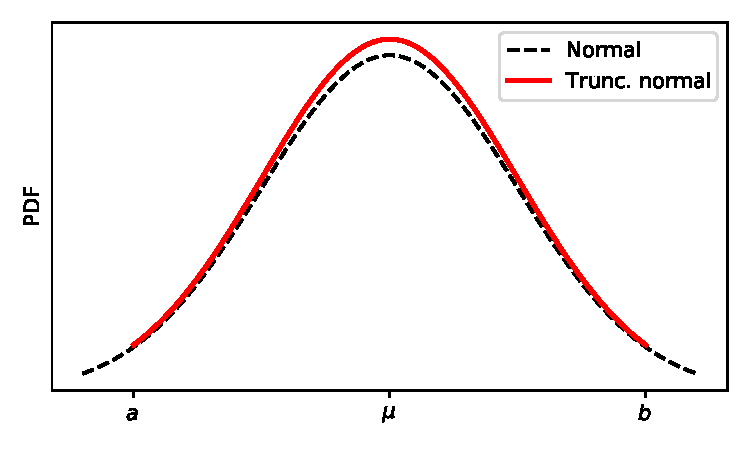
\includegraphics{solutions/unit07/unit07_ex2_PDF.pdf}
\caption{PDF of truncated normal}
\end{figure}

Compute the second non-central moment \(E[X^2]\) in four different ways:

\begin{enumerate}
\def\labelenumi{\arabic{enumi}.}
\item
  Use the fact that \(Var(X) = E[X^2] - E[X]^2\). Call the methods
  \texttt{mean()} and \texttt{var()} of the
  \href{https://docs.scipy.org/doc/scipy/reference/generated/scipy.stats.truncnorm.html}{truncated
  normal} implemented in SciPy to compute the (squared) mean and
  variance.

  \emph{Hint:} Import the truncated normal as follows:

\begin{verbatim}
from scipy.stats import truncnorm
\end{verbatim}
\item
  Use the \texttt{moment()} method of SciPy's truncated normal to
  directly compute the desired moment.
\item
  Use the \texttt{expect()} method of SciPy's truncated normal to
  compute the expectation \(E[X^2]\).
\item
  Use \href{https://en.wikipedia.org/wiki/Monte_Carlo_integration}{Monte
  Carlo integration} to compute the expectation \(E[X^2]\). There are
  numerous ways to do MC integration. In this exercise, we use a variant
  which draws random samples from a 2-dimensional uniform distribution
  to compute an area under the integrand:

  \begin{itemize}
  \tightlist
  \item
    To do this, define the integrand as
    \(x^2 \cdot f_t(x;a,b,\mu,\sigma)\) where \(f_t\) is the PDF of the
    truncated normal with parameters \(a\), \(b\), \(\mu\) and
    \(\sigma\).
  \item
    Draw random numbers in the rectangle which has length \(b-a\) and a
    height which is the maximum of the integrand on the integration
    interval \([a,b]\).
  \item
    Determine the fraction of sampled points that are below the
    integral, and use this to compute the area under the integrand.
  \end{itemize}

  The following figure illustrates this approach to integration. The
  blue dots are included in the integral whereas the red crosses are
  not:

  \begin{figure}
  \centering
  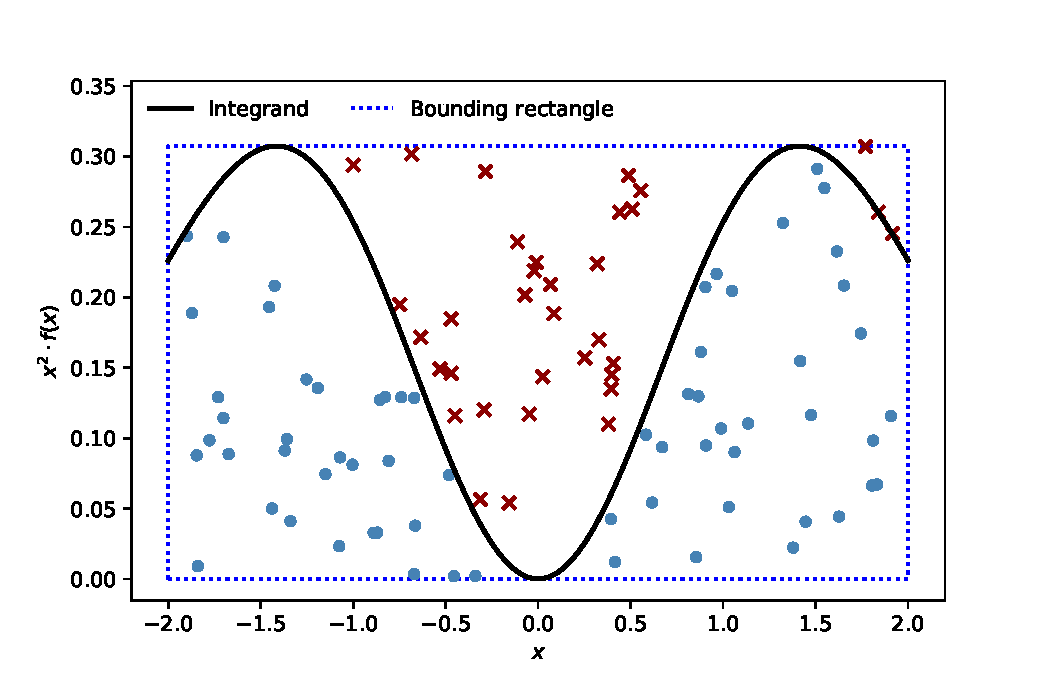
\includegraphics{solutions/unit07/unit07_ex2_MC.pdf}
  \caption{MC integration}
  \end{figure}

  This may not be the most practical way to do MC integration, and we
  will examine a more common approach in the next exercise.

  \emph{Note:} SciPy's truncated normal expects \emph{normalised}
  boundaries \(a\) and \(b\). Whenever the underlying distribution is
  \emph{not} standard normal, you have to pass \(z_a = (a-\mu)/\sigma\)
  and \(z_b = (b-\mu)/\sigma\) instead of \(a\) and \(b\) to all of
  \texttt{truncnorm}'s methods.
\end{enumerate}

    \hypertarget{exercise-3-multi-period-asset-returns}{%
\subsubsection{Exercise 3: Multi-period asset
returns}\label{exercise-3-multi-period-asset-returns}}

Consider an investor with initial assets \(a\) and a 2-period investment
horizon (we assume the investor does not change the asset position after
the first period).

Denote by \(R\) the total gross return over two periods, so that the
terminal wealth is given by \(W = a\cdot R\). The total gross return is
the product of the period-1 and period-2 gross returns,
\(R = R_1\cdot R_2\). We impose that per-period log returns
\(r_t = \log R_t\) are jointly normally distributed with mean
\(E[r_t] = \mu\), variance \(Var(r_t) = \sigma^2\) for \(t\in\{1,2\}\)
with a correlation coefficient \(Corr(r_1,r_2) = \rho\). Let \(a = 1\),
\(\mu = 0.04\), \(\sigma = 0.16\) and \(\rho = 0.5\).

\begin{enumerate}
\def\labelenumi{\arabic{enumi}.}
\item
  Derive the analytical expression for the expected total gross return
  after 2 periods.

  \emph{Hint:}

  \begin{itemize}
  \item
    Remember that since \((r_1,r_2)\) are jointly normally distributed,
    so is their sum, \(\log R = r_1 + r_2\).
  \item
    Moreover, if \(\log R\) is normally distributed with mean \(\mu_R\)
    and variance \(\sigma_R^2\), then \(R\) is
    \href{https://en.wikipedia.org/wiki/Log-normal_distribution}{log-normally}
    distributed and has the expected value

    \[E[R] = \exp\left(\mu_R + \frac{1}{2}\sigma_R^2 \right)\]
  \end{itemize}
\item
  Compute the expected terminal wealth after 2 periods using Monte Carlo
  simulation. To do this,

  \begin{enumerate}
  \def\labelenumii{\arabic{enumii}.}
  \item
    Draw \(N\) samples of multivariate normally distributed vectors
    \((r_{1i},r_{2i})\) using NumPy's
    \href{https://numpy.org/doc/stable/reference/random/generated/numpy.random.multivariate_normal.html}{multivariate\_normal()}.
  \item
    Compute the terminal wealth for each draw \(i\):
    \(W_i = a\exp(r_{1i})\exp(r_{2i})\).
  \item
    Compute the expected wealth as the sample average:

    \[E[W] \approx \overline{W} = \frac{1}{N}\sum_{i=1}^N W_i\]
  \end{enumerate}

  Make sure you get approximately the same result as in part 1 (you may
  need to increase the sample size if this is not the case).
\item
  Plot a histogram of the simulated total gross returns, and overlay it
  with the PDF of the log-normal distribution you derived in the first
  part.
\end{enumerate}

    \hypertarget{exercise-4-standard-error-and-increasing-sample-size}{%
\subsubsection{Exercise 4: Standard error and increasing sample
size}\label{exercise-4-standard-error-and-increasing-sample-size}}

Consider a setting in which we draw multiple samples indexed by \(k\)
such that these samples are increasing in the sample size \(N_k\), given
by \(N_k\) = 10, 50, 100, 500, 1000, 5000, 10000, 50000 and 100000.

The data for the \(k\)-th sample are \((x_{ik})_{i=1}^{N_k}\) where
\(i\) indexes some draw within the \(k\)-th sample. Assume that the data
are
\href{https://en.wikipedia.org/wiki/Log-normal_distribution}{log-normally}
distributed such that the underlying normal distribution has mean
\(\mu=0.5\) and variance \(\sigma^2 = 1.5^2\).

\begin{enumerate}
\def\labelenumi{\arabic{enumi}.}
\item
  For each sample size \(N_k\), use NumPy's
  \href{https://numpy.org/doc/stable/reference/random/generated/numpy.random.Generator.lognormal.html}{\texttt{lognormal()}}
  to draw a log-normally distributed sample.
\item
  For each sample, compute the sample mean and its standard error. As a
  reminder, the standard error of the \(k\)-th sample mean
  \(\overline{x}_k\) is defined as

  \[se(\overline{x}_k) = \sqrt{\frac{\widehat{\sigma}_{k}^2}{N_k}}\]

  where \(\widehat{\sigma}_{k}^2\) is the variance of residuals
  \(u_{ik} = x_{ik} - \overline{x}_k\) for each sample \(k\),

  \[\widehat{\sigma}_{k}^2 = \frac{1}{N_k-1}\sum_{i=1}^{N_k} u_{ik}^2\]
\item
  Plot the sample means for all samples, using the sample size on the
  \(x\)-axis and the estimated mean on the \(y\)-axis. Use the
  \(\log_{10}\) scale on the \(x\)-axis.

  \emph{Hint:} You can activate log scaling by calling
  \texttt{xscale(\textquotesingle{}log\textquotesingle{})}, or
  \texttt{set\_xscale(\textquotesingle{}log\textquotesingle{})} when
  using the object-oriented plotting interface.
\item
  Add a horizontal line showing the true mean (which is the same for all
  sample sizes).
\item
  Add confidence intervals (CI) for each sample size: use the interval
  \(\overline{x}_k \pm 2\times se(\overline{x}_k)\) to get a CI of
  approximately 95\%.
\end{enumerate}

    \hypertarget{exercise-5-the-jackknife}{%
\subsubsection{Exercise 5: The
jackknife}\label{exercise-5-the-jackknife}}

We continue with the setting from exercise 4, but instead of computing
the standard error as above, we now use a resampling technique known as
the \href{https://en.wikipedia.org/wiki/Jackknife_resampling}{jackknife}
to get the sample mean and its standard error.

\begin{enumerate}
\def\labelenumi{\arabic{enumi}.}
\tightlist
\item
  For each sample \(k\), compute \(N_k\) sample means
  \(\overline{x}_{-i,k}\) which are obtained by leaving out the \(i\)-th
  observation: \[
  \overline{x}_{-i,k} = \frac{1}{N_k-1}\sum_{j = 1, j \neq i}^{N_k} x_{jk} 
  \qquad i = 1,\dots,N_k
  \] where \(x_{jk}\) is the \(j\)-th draw in the \(k\)-th sample.
\item
  Compute the jackknife estimate of the sample mean as the average of
  these sub-sample means: \[
  \overline{x}_{k,jack} = \frac{1}{N_k}\sum_{i=1}^{N_k} \overline{x}_{-i,k}
  \] For the special case of a sample mean, it is straightforward to
  show that this is just the regular sample mean computed on the whole
  sample, \(\overline{x}_{k,jack} = \overline{x}_k\), where \[
  \overline{x}_k = \frac{1}{N_k}\sum_{i=1}^{N_k} x_{ik}
  \]
\item
  The jackknife estimate of the error variance for sample size \(N_k\)
  is then given by \[
  \begin{aligned}
  \widehat{var}(\overline{x}_k) 
      &= \frac{N_k - 1}{N_k} \sum_{i=1}^{N_k}\left(
              \overline{x}_{-i,k} - \overline{x}_{jack,k}\right)^2 \\
      &= \frac{1}{N_k(N_k-1)} \sum_{i=1}^{N_k}(x_{ik}-\overline{x}_k)^2
  \end{aligned}
  \] where the second line again follows as a special case if we are
  estimating the sample mean. The standard error of the sample mean is
  thus \[
  se(\overline{x}_k) = \sqrt{\widehat{var}(\overline{x}_k)}
  \]
\item
  Recreate the plot from exercise 4, but now use the jackknife estimate
  of the standard error instead.
\end{enumerate}

    \hypertarget{exercise-6-the-bootstrap}{%
\subsubsection{Exercise 6: The
bootstrap}\label{exercise-6-the-bootstrap}}

We continue with the setting from exercises 4 and 5, but now we use the
\href{https://en.wikipedia.org/wiki/Bootstrapping_(statistics)\#Case_resampling}{bootstrap}
to estimate the confidence intervals of the mean estimate.

\begin{enumerate}
\def\labelenumi{\arabic{enumi}.}
\tightlist
\item
  For each sample size \(N_k\) proceed as follows:

  \begin{enumerate}
  \def\labelenumii{\arabic{enumii}.}
  \tightlist
  \item
    Draw an initial sample of size \(N_k\) as before and compute the
    sample mean.
  \item
    Resample \(N_k\) observations by drawing from this initial sample
    \emph{with}\\
    \emph{replacement} using NumPy's
    \href{https://numpy.org/doc/stable/reference/random/generated/numpy.random.Generator.choice.html}{\texttt{choice()}}
    function.
  \item
    For each ``resample'', compute the sample mean. Say we have the
    \(j\)-th resample which consists of the draws
    \((x_{ik}^j)_{i=1}^{N_k}\), so we compute the \(j\)-th mean \[
    \overline{x}_{k}^j = \frac{1}{N_k} \sum_{i=1}^{N_k} x_{ik}^j
    \]
  \item
    Repeat steps 2 and 3 \(N_{bs} = 999\) times.
  \item
    Use these \(N_{bs}\) means to find the 2.5\% and 97.5\% percentiles
    of the mean estimate distribution, \(\overline{x}_k^{p2.5}\) and
    \(\overline{x}_k^{p97.5}\).
  \item
    The bootstrapped 95\% confidence interval is then given by
    \(\left[\overline{x}_k^{p2.5}, \overline{x}_k^{p97.5}\right]\).
  \end{enumerate}
\item
  Recreate the same plot as in exercises 4 and 5, but this time use the
  bootstrapped 95\% confidence interval you computed for each sample
  size.
\item
  For each sample size, store all bootstrapped means and use these to
  create a histogram of sample means. You will thus have to create 9
  histograms. Use vertical lines to indicate the 95\% confidence
  interval.
\end{enumerate}


\hypertarget{solutions}{%
\subsection{Solutions}\label{solutions}}

The solutions are also provided as Python scripts in the
\href{../lectures/solutions/unit7}{lectures/solutions/unit7/} folder.

    \hypertarget{solution-for-exercise-1}{%
\subsubsection{Solution for exercise 1}\label{solution-for-exercise-1}}

In the following solution, we create a figure with six panels (axes) and
iterate over these axes. In each iteration, we

\begin{enumerate}
\def\labelenumi{\arabic{enumi}.}
\tightlist
\item
  draw a random sample for the given (increasing) size;
\item
  plot the histogram using the current axes object; and
\item
  overlay the actual PDF.
\end{enumerate}

    \begin{tcolorbox}[breakable, size=fbox, boxrule=1pt, pad at break*=1mm,colback=cellbackground, colframe=cellborder]
\prompt{In}{incolor}{21}{\boxspacing}
\begin{Verbatim}[commandchars=\\\{\}]
\PY{k+kn}{import} \PY{n+nn}{matplotlib}\PY{n+nn}{.}\PY{n+nn}{pyplot} \PY{k}{as} \PY{n+nn}{plt}
\PY{k+kn}{import} \PY{n+nn}{numpy} \PY{k}{as} \PY{n+nn}{np}
\PY{k+kn}{from} \PY{n+nn}{numpy}\PY{n+nn}{.}\PY{n+nn}{random} \PY{k+kn}{import} \PY{n}{default\PYZus{}rng}
\PY{k+kn}{from} \PY{n+nn}{scipy}\PY{n+nn}{.}\PY{n+nn}{stats} \PY{k+kn}{import} \PY{n}{t} \PY{k}{as} \PY{n}{standard\PYZus{}t}

\PY{c+c1}{\PYZsh{} Sample sizes}
\PY{n}{Nobs} \PY{o}{=} \PY{n}{np}\PY{o}{.}\PY{n}{array}\PY{p}{(}\PY{p}{(}\PY{l+m+mi}{50}\PY{p}{,} \PY{l+m+mi}{100}\PY{p}{,} \PY{l+m+mi}{500}\PY{p}{,} \PY{l+m+mi}{1000}\PY{p}{,} \PY{l+m+mi}{5000}\PY{p}{,} \PY{l+m+mi}{10000}\PY{p}{)}\PY{p}{)}

\PY{c+c1}{\PYZsh{} degrees of freedom}
\PY{n}{df} \PY{o}{=} \PY{l+m+mi}{20}

\PY{c+c1}{\PYZsh{} Determine xlims such that we cover the (0.1, 99.9) percentiles}
\PY{c+c1}{\PYZsh{} of the distribution.}
\PY{n}{xmin}\PY{p}{,} \PY{n}{xmax} \PY{o}{=} \PY{n}{standard\PYZus{}t}\PY{o}{.}\PY{n}{ppf}\PY{p}{(}\PY{p}{(}\PY{l+m+mf}{0.001}\PY{p}{,} \PY{l+m+mf}{0.999}\PY{p}{)}\PY{p}{,} \PY{n}{df}\PY{o}{=}\PY{n}{df}\PY{p}{)}

\PY{n}{xvalues} \PY{o}{=} \PY{n}{np}\PY{o}{.}\PY{n}{linspace}\PY{p}{(}\PY{n}{xmin}\PY{p}{,} \PY{n}{xmax}\PY{p}{,} \PY{l+m+mi}{100}\PY{p}{)}
\PY{n}{pdf} \PY{o}{=} \PY{n}{standard\PYZus{}t}\PY{o}{.}\PY{n}{pdf}\PY{p}{(}\PY{n}{xvalues}\PY{p}{,} \PY{n}{df}\PY{o}{=}\PY{n}{df}\PY{p}{)}

\PY{n}{fig}\PY{p}{,} \PY{n}{ax} \PY{o}{=} \PY{n}{plt}\PY{o}{.}\PY{n}{subplots}\PY{p}{(}\PY{l+m+mi}{2}\PY{p}{,} \PY{l+m+mi}{3}\PY{p}{,} \PY{n}{sharex}\PY{o}{=}\PY{k+kc}{True}\PY{p}{,} \PY{n}{sharey}\PY{o}{=}\PY{k+kc}{True}\PY{p}{,} \PY{n}{figsize}\PY{o}{=}\PY{p}{(}\PY{l+m+mi}{12}\PY{p}{,} \PY{l+m+mi}{6}\PY{p}{)}\PY{p}{)}

\PY{c+c1}{\PYZsh{} initialize default RNG}
\PY{n}{rng} \PY{o}{=} \PY{n}{default\PYZus{}rng}\PY{p}{(}\PY{l+m+mi}{123}\PY{p}{)}

\PY{k}{for} \PY{n}{i}\PY{p}{,} \PY{n}{axes} \PY{o+ow}{in} \PY{n+nb}{enumerate}\PY{p}{(}\PY{n}{ax}\PY{o}{.}\PY{n}{flatten}\PY{p}{(}\PY{p}{)}\PY{p}{)}\PY{p}{:}
    \PY{c+c1}{\PYZsh{} Sample size to be plotted in current panel}
    \PY{n}{N} \PY{o}{=} \PY{n}{Nobs}\PY{p}{[}\PY{n}{i}\PY{p}{]}
    \PY{c+c1}{\PYZsh{} Draw sample of size N}
    \PY{n}{data} \PY{o}{=} \PY{n}{rng}\PY{o}{.}\PY{n}{standard\PYZus{}t}\PY{p}{(}\PY{n}{df}\PY{o}{=}\PY{n}{df}\PY{p}{,} \PY{n}{size}\PY{o}{=}\PY{n}{N}\PY{p}{)}

    \PY{c+c1}{\PYZsh{} plot histogram of given sample}
    \PY{n}{axes}\PY{o}{.}\PY{n}{hist}\PY{p}{(}\PY{n}{data}\PY{p}{,} \PY{n}{bins}\PY{o}{=}\PY{l+m+mi}{50}\PY{p}{,} \PY{n}{linewidth}\PY{o}{=}\PY{l+m+mf}{0.5}\PY{p}{,} \PY{n}{edgecolor}\PY{o}{=}\PY{l+s+s1}{\PYZsq{}}\PY{l+s+s1}{white}\PY{l+s+s1}{\PYZsq{}}\PY{p}{,} 
              \PY{n}{color}\PY{o}{=}\PY{l+s+s1}{\PYZsq{}}\PY{l+s+s1}{steelblue}\PY{l+s+s1}{\PYZsq{}}\PY{p}{,} \PY{n}{density}\PY{o}{=}\PY{k+kc}{True}\PY{p}{,} \PY{n}{label}\PY{o}{=}\PY{l+s+s1}{\PYZsq{}}\PY{l+s+s1}{Sample histogram}\PY{l+s+s1}{\PYZsq{}}\PY{p}{)}

    \PY{c+c1}{\PYZsh{} overlay actual PDF}
    \PY{n}{axes}\PY{o}{.}\PY{n}{plot}\PY{p}{(}\PY{n}{xvalues}\PY{p}{,} \PY{n}{pdf}\PY{p}{,} \PY{n}{color}\PY{o}{=}\PY{l+s+s1}{\PYZsq{}}\PY{l+s+s1}{red}\PY{l+s+s1}{\PYZsq{}}\PY{p}{,} \PY{n}{lw}\PY{o}{=}\PY{l+m+mf}{2.0}\PY{p}{,} \PY{n}{label}\PY{o}{=}\PY{l+s+s1}{\PYZsq{}}\PY{l+s+s1}{PDF}\PY{l+s+s1}{\PYZsq{}}\PY{p}{)}

    \PY{c+c1}{\PYZsh{} create text with current sample size}
    \PY{n}{axes}\PY{o}{.}\PY{n}{text}\PY{p}{(}\PY{l+m+mf}{0.05}\PY{p}{,} \PY{l+m+mf}{0.95}\PY{p}{,} \PY{l+s+sa}{f}\PY{l+s+s1}{\PYZsq{}}\PY{l+s+s1}{N=}\PY{l+s+si}{\PYZob{}}\PY{n}{N}\PY{l+s+si}{:}\PY{l+s+s1}{,d}\PY{l+s+si}{\PYZcb{}}\PY{l+s+s1}{\PYZsq{}}\PY{p}{,} \PY{n}{transform}\PY{o}{=}\PY{n}{axes}\PY{o}{.}\PY{n}{transAxes}\PY{p}{,} \PY{n}{va}\PY{o}{=}\PY{l+s+s1}{\PYZsq{}}\PY{l+s+s1}{top}\PY{l+s+s1}{\PYZsq{}}\PY{p}{)}

    \PY{n}{axes}\PY{o}{.}\PY{n}{set\PYZus{}xlim}\PY{p}{(}\PY{p}{(}\PY{n}{xmin}\PY{p}{,} \PY{n}{xmax}\PY{p}{)}\PY{p}{)}
    \PY{n}{axes}\PY{o}{.}\PY{n}{set\PYZus{}ylim}\PY{p}{(}\PY{p}{(}\PY{o}{\PYZhy{}}\PY{l+m+mf}{0.02}\PY{p}{,} \PY{l+m+mf}{1.3}\PY{p}{)}\PY{p}{)}

    \PY{c+c1}{\PYZsh{} plot legend only for the first panel}
    \PY{k}{if} \PY{n}{i} \PY{o}{==} \PY{l+m+mi}{0}\PY{p}{:}
        \PY{n}{axes}\PY{o}{.}\PY{n}{legend}\PY{p}{(}\PY{n}{loc}\PY{o}{=}\PY{l+s+s1}{\PYZsq{}}\PY{l+s+s1}{upper right}\PY{l+s+s1}{\PYZsq{}}\PY{p}{)}

\PY{c+c1}{\PYZsh{} compress space between individual panels}
\PY{n}{fig}\PY{o}{.}\PY{n}{tight\PYZus{}layout}\PY{p}{(}\PY{p}{)}
\PY{c+c1}{\PYZsh{} Add overall title}
\PY{n}{fig}\PY{o}{.}\PY{n}{suptitle}\PY{p}{(}\PY{l+s+s1}{\PYZsq{}}\PY{l+s+s1}{Draws from the standard\PYZhy{}t distribution}\PY{l+s+s1}{\PYZsq{}}\PY{p}{,} \PY{n}{fontsize}\PY{o}{=}\PY{l+m+mi}{16}\PY{p}{,} \PY{n}{y}\PY{o}{=}\PY{l+m+mf}{1.05}\PY{p}{)}
    
\end{Verbatim}
\end{tcolorbox}

            \begin{tcolorbox}[breakable, size=fbox, boxrule=.5pt, pad at break*=1mm, opacityfill=0]
\prompt{Out}{outcolor}{21}{\boxspacing}
\begin{Verbatim}[commandchars=\\\{\}]
Text(0.5, 1.05, 'Draws from the standard-t distribution')
\end{Verbatim}
\end{tcolorbox}
        
    \begin{center}
    \adjustimage{max size={0.9\linewidth}{0.9\paperheight}}{unit07_files/unit07_53_1.pdf}
    \end{center}
    { \hspace*{\fill} \\}
    
    A few comments on how we create the \(x\)-values and the plot range for
these graphs:

\begin{enumerate}
\def\labelenumi{\arabic{enumi}.}
\tightlist
\item
  In principle, we could draw arbitrarily large or small realised
  values, but we want to restrict the plot limits to a reasonable
  interval.
\item
  To find such an interval, we compute the percentiles corresponding to
  0.1\% and 99.9\%, which will cover almost any point we'd want to plot.
\item
  Moreover, we need to compute the \(x\)-values and evaluate the PDF at
  these points only once since these will remain unchanged for all
  sample sizes.
\end{enumerate}

Note also that the \texttt{subplots()} function returns a 2-dimensional
array (since we requested a \(2 \times 3\) layout). We iterate over the
\emph{flattened} array of axes objects instead of writing two nested
loops over rows and columns.

    \hypertarget{solution-for-exercise-2}{%
\subsubsection{Solution for exercise 2}\label{solution-for-exercise-2}}

Computing the second non-central moment using the first three methods is
straightforward. All you need to do is to make sure that you pass the
correct parameters to SciPy's \texttt{truncnorm} methods:

    \begin{tcolorbox}[breakable, size=fbox, boxrule=1pt, pad at break*=1mm,colback=cellbackground, colframe=cellborder]
\prompt{In}{incolor}{22}{\boxspacing}
\begin{Verbatim}[commandchars=\\\{\}]
\PY{k+kn}{import} \PY{n+nn}{numpy} \PY{k}{as} \PY{n+nn}{np}
\PY{k+kn}{from} \PY{n+nn}{scipy}\PY{n+nn}{.}\PY{n+nn}{stats} \PY{k+kn}{import} \PY{n}{truncnorm}

\PY{c+c1}{\PYZsh{} Parameters}
\PY{n}{mu} \PY{o}{=} \PY{l+m+mf}{0.0}
\PY{n}{sigma} \PY{o}{=} \PY{l+m+mf}{1.0}
\PY{n}{a} \PY{o}{=} \PY{n}{mu} \PY{o}{\PYZhy{}} \PY{l+m+mi}{2}\PY{o}{*}\PY{n}{sigma}
\PY{n}{b} \PY{o}{=} \PY{n}{mu} \PY{o}{+} \PY{l+m+mi}{2}\PY{o}{*}\PY{n}{sigma}

\PY{c+c1}{\PYZsh{} Standardised boundaries if underlying non\PYZhy{}truncated distr. is}
\PY{c+c1}{\PYZsh{} NOT standard normal}
\PY{n}{za} \PY{o}{=} \PY{p}{(}\PY{n}{a}\PY{o}{\PYZhy{}}\PY{n}{mu}\PY{p}{)}\PY{o}{/}\PY{n}{sigma}
\PY{n}{zb} \PY{o}{=} \PY{p}{(}\PY{n}{b}\PY{o}{\PYZhy{}}\PY{n}{mu}\PY{p}{)}\PY{o}{/}\PY{n}{sigma}

\PY{c+c1}{\PYZsh{} Method 1: Compute from E[X\PYZca{}2] = Var(X) + E[X]\PYZca{}2}
\PY{n}{var} \PY{o}{=} \PY{n}{truncnorm}\PY{o}{.}\PY{n}{var}\PY{p}{(}\PY{n}{za}\PY{p}{,} \PY{n}{zb}\PY{p}{,} \PY{n}{loc}\PY{o}{=}\PY{n}{mu}\PY{p}{,} \PY{n}{scale}\PY{o}{=}\PY{n}{sigma}\PY{p}{)}
\PY{n}{mean} \PY{o}{=} \PY{n}{truncnorm}\PY{o}{.}\PY{n}{mean}\PY{p}{(}\PY{n}{za}\PY{p}{,} \PY{n}{zb}\PY{p}{,} \PY{n}{loc}\PY{o}{=}\PY{n}{mu}\PY{p}{,} \PY{n}{scale}\PY{o}{=}\PY{n}{sigma}\PY{p}{)}
\PY{n}{m2\PYZus{}var\PYZus{}mean} \PY{o}{=} \PY{n}{var} \PY{o}{+} \PY{n}{mean} \PY{o}{*}\PY{o}{*} \PY{l+m+mf}{2.0}

\PY{c+c1}{\PYZsh{} Method 2: Compute using moment()}
\PY{n}{m2} \PY{o}{=} \PY{n}{truncnorm}\PY{o}{.}\PY{n}{moment}\PY{p}{(}\PY{l+m+mi}{2}\PY{p}{,} \PY{n}{za}\PY{p}{,} \PY{n}{zb}\PY{p}{,} \PY{n}{loc}\PY{o}{=}\PY{n}{mu}\PY{p}{,} \PY{n}{scale}\PY{o}{=}\PY{n}{sigma}\PY{p}{)}

\PY{c+c1}{\PYZsh{} Method 3: Compute moment using expect() function}
\PY{n}{m2\PYZus{}expect} \PY{o}{=} \PY{n}{truncnorm}\PY{o}{.}\PY{n}{expect}\PY{p}{(}\PY{k}{lambda} \PY{n}{x}\PY{p}{:} \PY{n}{x}\PY{o}{*}\PY{o}{*}\PY{l+m+mf}{2.0}\PY{p}{,} \PY{n}{args}\PY{o}{=}\PY{p}{(}\PY{n}{za}\PY{p}{,} \PY{n}{zb}\PY{p}{)}\PY{p}{,} 
                             \PY{n}{loc}\PY{o}{=}\PY{n}{mu}\PY{p}{,} \PY{n}{scale}\PY{o}{=}\PY{n}{sigma}\PY{p}{)}

\PY{n+nb}{print}\PY{p}{(}\PY{l+s+sa}{f}\PY{l+s+s1}{\PYZsq{}}\PY{l+s+s1}{Second non\PYZhy{}central moment, var + mean\PYZca{}2: }\PY{l+s+si}{\PYZob{}}\PY{n}{m2\PYZus{}var\PYZus{}mean}\PY{l+s+si}{:}\PY{l+s+s1}{.5e}\PY{l+s+si}{\PYZcb{}}\PY{l+s+s1}{\PYZsq{}}\PY{p}{)}
\PY{n+nb}{print}\PY{p}{(}\PY{l+s+sa}{f}\PY{l+s+s1}{\PYZsq{}}\PY{l+s+s1}{Second non\PYZhy{}central moment, moment(): }\PY{l+s+si}{\PYZob{}}\PY{n}{m2}\PY{l+s+si}{:}\PY{l+s+s1}{.5e}\PY{l+s+si}{\PYZcb{}}\PY{l+s+s1}{\PYZsq{}}\PY{p}{)}
\PY{n+nb}{print}\PY{p}{(}\PY{l+s+sa}{f}\PY{l+s+s1}{\PYZsq{}}\PY{l+s+s1}{Second non\PYZhy{}central moment, expect(): }\PY{l+s+si}{\PYZob{}}\PY{n}{m2\PYZus{}expect}\PY{l+s+si}{:}\PY{l+s+s1}{.5e}\PY{l+s+si}{\PYZcb{}}\PY{l+s+s1}{\PYZsq{}}\PY{p}{)}
\end{Verbatim}
\end{tcolorbox}

    \begin{Verbatim}[commandchars=\\\{\}]
Second non-central moment, var + mean\^{}2: 7.73741e-01
Second non-central moment, moment(): 7.73741e-01
Second non-central moment, expect(): 7.73741e-01
    \end{Verbatim}

    The fourth method is more involved. We first define the integrand as
follows:

    \begin{tcolorbox}[breakable, size=fbox, boxrule=1pt, pad at break*=1mm,colback=cellbackground, colframe=cellborder]
\prompt{In}{incolor}{23}{\boxspacing}
\begin{Verbatim}[commandchars=\\\{\}]
\PY{c+c1}{\PYZsh{} Function to compute integrand}
\PY{k}{def} \PY{n+nf}{f\PYZus{}integrand}\PY{p}{(}\PY{n}{x}\PY{p}{,} \PY{n}{a}\PY{p}{,} \PY{n}{b}\PY{p}{,} \PY{n}{mu}\PY{p}{,} \PY{n}{sigma}\PY{p}{)}\PY{p}{:}
    \PY{c+c1}{\PYZsh{} Transform to boundaries required by SciPy\PYZsq{}s truncnorm}
    \PY{n}{za} \PY{o}{=} \PY{p}{(}\PY{n}{a} \PY{o}{\PYZhy{}} \PY{n}{mu}\PY{p}{)} \PY{o}{/} \PY{n}{sigma}
    \PY{n}{zb} \PY{o}{=} \PY{p}{(}\PY{n}{b} \PY{o}{\PYZhy{}} \PY{n}{mu}\PY{p}{)} \PY{o}{/} \PY{n}{sigma}
    \PY{c+c1}{\PYZsh{} Evaluate truncated normal PDF}
    \PY{n}{pdf} \PY{o}{=} \PY{n}{truncnorm}\PY{o}{.}\PY{n}{pdf}\PY{p}{(}\PY{n}{x}\PY{p}{,} \PY{n}{za}\PY{p}{,} \PY{n}{zb}\PY{p}{,} \PY{n}{loc}\PY{o}{=}\PY{n}{mu}\PY{p}{,} \PY{n}{scale}\PY{o}{=}\PY{n}{sigma}\PY{p}{)}
    \PY{c+c1}{\PYZsh{} Compute integrand x\PYZca{}2 * f(x)}
    \PY{n}{result} \PY{o}{=} \PY{n}{x} \PY{o}{*}\PY{o}{*} \PY{l+m+mf}{2.0} \PY{o}{*} \PY{n}{pdf}
    \PY{k}{return} \PY{n}{result}
\end{Verbatim}
\end{tcolorbox}

    The remainder of the Monte Carlo code look as follows:

    \begin{tcolorbox}[breakable, size=fbox, boxrule=1pt, pad at break*=1mm,colback=cellbackground, colframe=cellborder]
\prompt{In}{incolor}{24}{\boxspacing}
\begin{Verbatim}[commandchars=\\\{\}]
\PY{k+kn}{from} \PY{n+nn}{numpy}\PY{n+nn}{.}\PY{n+nn}{random} \PY{k+kn}{import} \PY{n}{default\PYZus{}rng}

\PY{c+c1}{\PYZsh{} Initialise RNG}
\PY{n}{rng} \PY{o}{=} \PY{n}{default\PYZus{}rng}\PY{p}{(}\PY{l+m+mi}{123}\PY{p}{)}
\PY{c+c1}{\PYZsh{} Sample size for Monte Carlo integration}
\PY{n}{Nsample} \PY{o}{=} \PY{l+m+mi}{50000}

\PY{c+c1}{\PYZsh{} x\PYZhy{}values should be uniformly distributed on [a, b]}
\PY{n}{xsample} \PY{o}{=} \PY{n}{rng}\PY{o}{.}\PY{n}{uniform}\PY{p}{(}\PY{n}{a}\PY{p}{,} \PY{n}{b}\PY{p}{,} \PY{n}{size}\PY{o}{=}\PY{n}{Nsample}\PY{p}{)}
\PY{c+c1}{\PYZsh{} Alternatively we can also just use equidistant x\PYZhy{}values, in}
\PY{c+c1}{\PYZsh{} low\PYZhy{}dimensional problems it makes no difference.}
\PY{c+c1}{\PYZsh{} xsample = np.linspace(a, b, Nsamples)}

\PY{c+c1}{\PYZsh{} Evaluate integrand at sampled x\PYZhy{}values}
\PY{n}{integrand} \PY{o}{=} \PY{n}{f\PYZus{}integrand}\PY{p}{(}\PY{n}{xsample}\PY{p}{,} \PY{n}{a}\PY{p}{,} \PY{n}{b}\PY{p}{,} \PY{n}{mu}\PY{p}{,} \PY{n}{sigma}\PY{p}{)}

\PY{c+c1}{\PYZsh{} Compute size of bounding rectangle:}
\PY{c+c1}{\PYZsh{} the height is taken as the largest realisation of the integrand.}
\PY{n}{length} \PY{o}{=} \PY{n}{b} \PY{o}{\PYZhy{}} \PY{n}{a}
\PY{n}{height} \PY{o}{=} \PY{n}{np}\PY{o}{.}\PY{n}{amax}\PY{p}{(}\PY{n}{integrand}\PY{p}{)}
\PY{n}{area} \PY{o}{=} \PY{n}{height} \PY{o}{*} \PY{n}{length}
\PY{c+c1}{\PYZsh{} draw y\PYZhy{}values from uniform distribution on [0, height]}
\PY{n}{ysample} \PY{o}{=} \PY{n}{rng}\PY{o}{.}\PY{n}{uniform}\PY{p}{(}\PY{l+m+mi}{0}\PY{p}{,} \PY{n}{height}\PY{p}{,} \PY{n}{size}\PY{o}{=}\PY{n}{Nsample}\PY{p}{)}
\PY{c+c1}{\PYZsh{} Compute fraction of points that are underneath the PDF}
\PY{n}{frac} \PY{o}{=} \PY{n}{np}\PY{o}{.}\PY{n}{mean}\PY{p}{(}\PY{n}{ysample} \PY{o}{\PYZlt{}}\PY{o}{=} \PY{n}{integrand}\PY{p}{)}
\PY{n}{integral\PYZus{}MC} \PY{o}{=} \PY{n}{frac} \PY{o}{*} \PY{n}{area}

\PY{n+nb}{print}\PY{p}{(}\PY{l+s+sa}{f}\PY{l+s+s1}{\PYZsq{}}\PY{l+s+s1}{Second non\PYZhy{}central moment, MC integration: }\PY{l+s+si}{\PYZob{}}\PY{n}{integral\PYZus{}MC}\PY{l+s+si}{:}\PY{l+s+s1}{.5e}\PY{l+s+si}{\PYZcb{}}\PY{l+s+s1}{\PYZsq{}}\PY{p}{)}
\end{Verbatim}
\end{tcolorbox}

    \begin{Verbatim}[commandchars=\\\{\}]
Second non-central moment, MC integration: 7.72828e-01
    \end{Verbatim}

    You might have noticed that MC integration is not the fastest to
converge, but using 50000 draws is sufficient to get somewhat close to
the other three methods.

In this case we do not actually need Monte Carlo methods, because the
dimensionality of the problem is so low. We could just as well have used
a dense deterministic rectangular grid instead of randomly-drawn points.

The entire Python script which also generates the graphs displayed in
the exercise can be found in the
\href{../lectures/solutions/unit7}{solutions} folder

    \hypertarget{solution-for-exercise-3}{%
\subsubsection{Solution for exercise 3}\label{solution-for-exercise-3}}

\textbf{Part 1}

The first part is purely analytical. We use it to verify that the code
in part 2 yields the correct result.

Since \((r_1, r_2)\) are jointly normal, a standard result is that their
sum \(r_1 + r_2\) is normally distributed with mean and variance given
by

\[\mu_{rr} = E[r_1 + r_2] = 2\mu \]

\[
\sigma^2_{rr} = Var(r_1+r_2) = Var(r_1) + Var(r_2) + 2\cdot Cov(r_1,r_2) = 2\sigma^2 + 2\rho\sigma^2 
\]

This is even simpler than the usual formulas since both per-period log
returns have the same mean and variance.

Moreover, since \(\log R = r_1 + r_2\) is normally distributed, \(R\) is
log-normally distributed and has the expected value \[
E[R] = \exp\left(\mu_{rr} + \frac{1}{2}\sigma_{rr}^2 \right)
    = \exp\left(2\mu + (1+\rho) \sigma^2 \right)
\] Since \(a = 1\), this is also the expected value of terminal wealth
\(W\).

We can plug in the parameter values to compute the numerical value:

    \begin{tcolorbox}[breakable, size=fbox, boxrule=1pt, pad at break*=1mm,colback=cellbackground, colframe=cellborder]
\prompt{In}{incolor}{25}{\boxspacing}
\begin{Verbatim}[commandchars=\\\{\}]
\PY{k+kn}{import} \PY{n+nn}{numpy} \PY{k}{as} \PY{n+nn}{np}

\PY{c+c1}{\PYZsh{} Parameters}
\PY{n}{a} \PY{o}{=} \PY{l+m+mf}{1.0}                         \PY{c+c1}{\PYZsh{} Initial assets}
\PY{n}{mu} \PY{o}{=} \PY{n}{np}\PY{o}{.}\PY{n}{array}\PY{p}{(}\PY{p}{(}\PY{l+m+mf}{0.04}\PY{p}{,} \PY{l+m+mf}{0.04}\PY{p}{)}\PY{p}{)}     \PY{c+c1}{\PYZsh{} average log returns}
\PY{n}{sigma} \PY{o}{=} \PY{l+m+mf}{0.16}                    \PY{c+c1}{\PYZsh{} std. dev. of log returns}
\PY{n}{rho} \PY{o}{=} \PY{l+m+mf}{0.5}                       \PY{c+c1}{\PYZsh{} serial correlation}

\PY{c+c1}{\PYZsh{} Exact expectation}
\PY{n}{var\PYZus{}rr} \PY{o}{=} \PY{l+m+mf}{2.0} \PY{o}{*} \PY{n}{sigma} \PY{o}{*}\PY{o}{*} \PY{l+m+mf}{2.0} \PY{o}{+} \PY{l+m+mf}{2.0} \PY{o}{*} \PY{n}{rho} \PY{o}{*} \PY{n}{sigma} \PY{o}{*}\PY{o}{*} \PY{l+m+mf}{2.0}
\PY{n}{sigma\PYZus{}rr} \PY{o}{=} \PY{n}{np}\PY{o}{.}\PY{n}{sqrt}\PY{p}{(}\PY{n}{var\PYZus{}rr}\PY{p}{)}
\PY{n}{mu\PYZus{}rr} \PY{o}{=} \PY{n}{np}\PY{o}{.}\PY{n}{sum}\PY{p}{(}\PY{n}{mu}\PY{p}{)}

\PY{n}{exp\PYZus{}exact} \PY{o}{=} \PY{n}{a} \PY{o}{*} \PY{n}{np}\PY{o}{.}\PY{n}{exp}\PY{p}{(}\PY{n}{mu\PYZus{}rr} \PY{o}{+} \PY{n}{sigma\PYZus{}rr} \PY{o}{*}\PY{o}{*} \PY{l+m+mf}{2.0} \PY{o}{/} \PY{l+m+mf}{2.0}\PY{p}{)}

\PY{n+nb}{print}\PY{p}{(}\PY{l+s+sa}{f}\PY{l+s+s1}{\PYZsq{}}\PY{l+s+s1}{Expected portfolio value (exact): }\PY{l+s+si}{\PYZob{}}\PY{n}{exp\PYZus{}exact}\PY{l+s+si}{:}\PY{l+s+s1}{.4f}\PY{l+s+si}{\PYZcb{}}\PY{l+s+s1}{\PYZsq{}}\PY{p}{)}
\end{Verbatim}
\end{tcolorbox}

    \begin{Verbatim}[commandchars=\\\{\}]
Expected portfolio value (exact): 1.1257
    \end{Verbatim}

    \textbf{Parts 2 and 3}

To perform the Monte Carlo simulation, we need to define the vector of
means and the variance-covariance matrix which we can pass to NumPy's
\texttt{multivariate\_normal()} to sample returns \((r_1, r_2)\):

    \begin{tcolorbox}[breakable, size=fbox, boxrule=1pt, pad at break*=1mm,colback=cellbackground, colframe=cellborder]
\prompt{In}{incolor}{26}{\boxspacing}
\begin{Verbatim}[commandchars=\\\{\}]
\PY{k+kn}{import} \PY{n+nn}{numpy} \PY{k}{as} \PY{n+nn}{np}
\PY{k+kn}{from} \PY{n+nn}{numpy}\PY{n+nn}{.}\PY{n+nn}{random} \PY{k+kn}{import} \PY{n}{default\PYZus{}rng}
\PY{k+kn}{from} \PY{n+nn}{scipy}\PY{n+nn}{.}\PY{n+nn}{stats} \PY{k+kn}{import} \PY{n}{lognorm}

\PY{c+c1}{\PYZsh{} Parameters}
\PY{n}{a} \PY{o}{=} \PY{l+m+mf}{1.0}                         \PY{c+c1}{\PYZsh{} Initial assets}
\PY{n}{mu} \PY{o}{=} \PY{n}{np}\PY{o}{.}\PY{n}{array}\PY{p}{(}\PY{p}{(}\PY{l+m+mf}{0.04}\PY{p}{,} \PY{l+m+mf}{0.04}\PY{p}{)}\PY{p}{)}     \PY{c+c1}{\PYZsh{} average log returns}
\PY{n}{sigma} \PY{o}{=} \PY{l+m+mf}{0.16}                    \PY{c+c1}{\PYZsh{} std. dev. of log returns}
\PY{n}{rho} \PY{o}{=} \PY{l+m+mf}{0.5}                       \PY{c+c1}{\PYZsh{} serial correlation}

\PY{c+c1}{\PYZsh{} Covariance}
\PY{n}{cov} \PY{o}{=} \PY{n}{rho}\PY{o}{*}\PY{n}{sigma}\PY{o}{*}\PY{o}{*}\PY{l+m+mf}{2.0}
\PY{c+c1}{\PYZsh{} variance\PYZhy{}covariance matrix}
\PY{n}{vcv} \PY{o}{=} \PY{n}{np}\PY{o}{.}\PY{n}{array}\PY{p}{(}\PY{p}{[}\PY{p}{[}\PY{n}{sigma}\PY{o}{*}\PY{o}{*}\PY{l+m+mf}{2.0}\PY{p}{,} \PY{n}{cov}\PY{p}{]}\PY{p}{,}
                \PY{p}{[}\PY{n}{cov}\PY{p}{,} \PY{n}{sigma}\PY{o}{*}\PY{o}{*}\PY{l+m+mf}{2.0}\PY{p}{]}\PY{p}{]}\PY{p}{)}

\PY{n}{Nsample} \PY{o}{=} \PY{l+m+mi}{5000000}
\PY{n}{rng} \PY{o}{=} \PY{n}{default\PYZus{}rng}\PY{p}{(}\PY{l+m+mi}{123}\PY{p}{)}
\PY{c+c1}{\PYZsh{} Draw MV normal samples: each row corresponds to one draw}
\PY{n}{samples} \PY{o}{=} \PY{n}{rng}\PY{o}{.}\PY{n}{multivariate\PYZus{}normal}\PY{p}{(}\PY{n}{mean}\PY{o}{=}\PY{n}{mu}\PY{p}{,} \PY{n}{cov}\PY{o}{=}\PY{n}{vcv}\PY{p}{,} \PY{n}{size}\PY{o}{=}\PY{n}{Nsample}\PY{p}{)}

\PY{c+c1}{\PYZsh{} Evaluate total gross return at sampled points:}
\PY{c+c1}{\PYZsh{}   R = exp(r\PYZus{}1) * exp(r\PYZus{}2)}
\PY{n}{returns} \PY{o}{=} \PY{n}{np}\PY{o}{.}\PY{n}{prod}\PY{p}{(}\PY{n}{np}\PY{o}{.}\PY{n}{exp}\PY{p}{(}\PY{n}{samples}\PY{p}{)}\PY{p}{,} \PY{n}{axis}\PY{o}{=}\PY{l+m+mi}{1}\PY{p}{)}
\PY{c+c1}{\PYZsh{} Sampled terminal wealth after 2 periods}
\PY{n}{wealth} \PY{o}{=} \PY{n}{a} \PY{o}{*} \PY{n}{returns}
\PY{c+c1}{\PYZsh{} Expected terminal wealth}
\PY{n}{exp\PYZus{}MC} \PY{o}{=} \PY{n}{np}\PY{o}{.}\PY{n}{mean}\PY{p}{(}\PY{n}{wealth}\PY{p}{)}

\PY{n+nb}{print}\PY{p}{(}\PY{l+s+sa}{f}\PY{l+s+s1}{\PYZsq{}}\PY{l+s+s1}{Expected portfolio value (MC): }\PY{l+s+si}{\PYZob{}}\PY{n}{exp\PYZus{}MC}\PY{l+s+si}{:}\PY{l+s+s1}{.4f}\PY{l+s+si}{\PYZcb{}}\PY{l+s+s1}{\PYZsq{}}\PY{p}{)}
\end{Verbatim}
\end{tcolorbox}

    \begin{Verbatim}[commandchars=\\\{\}]
Expected portfolio value (MC): 1.1256
    \end{Verbatim}

    Finally, we use the sampled points and the \texttt{pdf()} method of
SciPy's
\href{https://docs.scipy.org/doc/scipy/reference/generated/scipy.stats.lognorm.html}{lognorm}
to plot the histogram and the true PDF.

    \begin{tcolorbox}[breakable, size=fbox, boxrule=1pt, pad at break*=1mm,colback=cellbackground, colframe=cellborder]
\prompt{In}{incolor}{27}{\boxspacing}
\begin{Verbatim}[commandchars=\\\{\}]
\PY{k+kn}{import} \PY{n+nn}{matplotlib}\PY{n+nn}{.}\PY{n+nn}{pyplot} \PY{k}{as} \PY{n+nn}{plt}

\PY{n}{fig}\PY{p}{,} \PY{n}{ax} \PY{o}{=} \PY{n}{plt}\PY{o}{.}\PY{n}{subplots}\PY{p}{(}\PY{l+m+mi}{1}\PY{p}{,} \PY{l+m+mi}{1}\PY{p}{)}

\PY{n}{ax}\PY{o}{.}\PY{n}{hist}\PY{p}{(}\PY{n}{returns}\PY{p}{,} \PY{n}{bins}\PY{o}{=}\PY{l+m+mi}{75}\PY{p}{,} \PY{n}{density}\PY{o}{=}\PY{k+kc}{True}\PY{p}{,} \PY{n}{color}\PY{o}{=}\PY{l+s+s1}{\PYZsq{}}\PY{l+s+s1}{steelblue}\PY{l+s+s1}{\PYZsq{}}\PY{p}{,} \PY{n}{lw}\PY{o}{=}\PY{l+m+mf}{0.5}\PY{p}{,}
        \PY{n}{edgecolor}\PY{o}{=}\PY{l+s+s1}{\PYZsq{}}\PY{l+s+s1}{white}\PY{l+s+s1}{\PYZsq{}}\PY{p}{,} \PY{n}{alpha}\PY{o}{=}\PY{l+m+mf}{.8}\PY{p}{,} \PY{n}{label}\PY{o}{=}\PY{l+s+s1}{\PYZsq{}}\PY{l+s+s1}{Sample}\PY{l+s+s1}{\PYZsq{}}\PY{p}{)}

\PY{c+c1}{\PYZsh{} Plot log\PYZhy{}normal PDF of total gross return}
\PY{n}{xmin}\PY{p}{,} \PY{n}{xmax} \PY{o}{=} \PY{n}{np}\PY{o}{.}\PY{n}{amin}\PY{p}{(}\PY{n}{returns}\PY{p}{)}\PY{p}{,} \PY{n}{np}\PY{o}{.}\PY{n}{amax}\PY{p}{(}\PY{n}{returns}\PY{p}{)}
\PY{n}{xvalues} \PY{o}{=} \PY{n}{np}\PY{o}{.}\PY{n}{linspace}\PY{p}{(}\PY{n}{xmin}\PY{p}{,} \PY{n}{xmax}\PY{p}{,} \PY{l+m+mi}{200}\PY{p}{)}
\PY{n}{pdf} \PY{o}{=} \PY{n}{lognorm}\PY{o}{.}\PY{n}{pdf}\PY{p}{(}\PY{n}{xvalues}\PY{p}{,} \PY{n}{s}\PY{o}{=}\PY{n}{sigma\PYZus{}rr}\PY{p}{,} \PY{n}{loc}\PY{o}{=}\PY{n}{mu\PYZus{}rr}\PY{p}{)}
\PY{n}{ax}\PY{o}{.}\PY{n}{plot}\PY{p}{(}\PY{n}{xvalues}\PY{p}{,} \PY{n}{pdf}\PY{p}{,} \PY{n}{c}\PY{o}{=}\PY{l+s+s1}{\PYZsq{}}\PY{l+s+s1}{red}\PY{l+s+s1}{\PYZsq{}}\PY{p}{,} \PY{n}{lw}\PY{o}{=}\PY{l+m+mf}{1.5}\PY{p}{,} \PY{n}{label}\PY{o}{=}\PY{l+s+s1}{\PYZsq{}}\PY{l+s+s1}{PDF}\PY{l+s+s1}{\PYZsq{}}\PY{p}{)}

\PY{c+c1}{\PYZsh{} Add line with true expected value}
\PY{n}{ax}\PY{o}{.}\PY{n}{axvline}\PY{p}{(}\PY{n}{exp\PYZus{}exact}\PY{p}{,} \PY{n}{lw}\PY{o}{=}\PY{l+m+mf}{1.0}\PY{p}{,} \PY{n}{color}\PY{o}{=}\PY{l+s+s1}{\PYZsq{}}\PY{l+s+s1}{black}\PY{l+s+s1}{\PYZsq{}}\PY{p}{,} \PY{n}{ls}\PY{o}{=}\PY{l+s+s1}{\PYZsq{}}\PY{l+s+s1}{\PYZhy{}\PYZhy{}}\PY{l+s+s1}{\PYZsq{}}\PY{p}{,} \PY{n}{label}\PY{o}{=}\PY{l+s+s1}{\PYZsq{}}\PY{l+s+s1}{Mean}\PY{l+s+s1}{\PYZsq{}}\PY{p}{)}

\PY{n}{ax}\PY{o}{.}\PY{n}{set\PYZus{}xlabel}\PY{p}{(}\PY{l+s+s1}{\PYZsq{}}\PY{l+s+s1}{Total gross return \PYZdl{}R\PYZdl{}}\PY{l+s+s1}{\PYZsq{}}\PY{p}{)}
\PY{n}{ax}\PY{o}{.}\PY{n}{set\PYZus{}ylabel}\PY{p}{(}\PY{l+s+s1}{\PYZsq{}}\PY{l+s+s1}{Density}\PY{l+s+s1}{\PYZsq{}}\PY{p}{)}
\PY{n}{ax}\PY{o}{.}\PY{n}{legend}\PY{p}{(}\PY{n}{loc}\PY{o}{=}\PY{l+s+s1}{\PYZsq{}}\PY{l+s+s1}{upper right}\PY{l+s+s1}{\PYZsq{}}\PY{p}{,} \PY{n}{frameon}\PY{o}{=}\PY{k+kc}{False}\PY{p}{)}
\end{Verbatim}
\end{tcolorbox}

            \begin{tcolorbox}[breakable, size=fbox, boxrule=.5pt, pad at break*=1mm, opacityfill=0]
\prompt{Out}{outcolor}{27}{\boxspacing}
\begin{Verbatim}[commandchars=\\\{\}]
<matplotlib.legend.Legend at 0x7fe64c7ed660>
\end{Verbatim}
\end{tcolorbox}
        
    \begin{center}
    \adjustimage{max size={0.9\linewidth}{0.9\paperheight}}{unit07_files/unit07_67_1.pdf}
    \end{center}
    { \hspace*{\fill} \\}
    
    The dashed black line shows the analytically derived expected total
gross return.

    \hypertarget{solution-for-exercise-4}{%
\subsubsection{Solution for exercise 4}\label{solution-for-exercise-4}}

We solve the exercise by iterating over all sample sizes, drawing a new
log-normal sample and computing the sample mean and standard error.
These are stored in the arrays \texttt{mean\_hat} and \texttt{std\_err},
which we then use the generate the plot.

    \begin{tcolorbox}[breakable, size=fbox, boxrule=1pt, pad at break*=1mm,colback=cellbackground, colframe=cellborder]
\prompt{In}{incolor}{28}{\boxspacing}
\begin{Verbatim}[commandchars=\\\{\}]
\PY{k+kn}{import} \PY{n+nn}{numpy} \PY{k}{as} \PY{n+nn}{np}
\PY{k+kn}{from} \PY{n+nn}{numpy}\PY{n+nn}{.}\PY{n+nn}{random} \PY{k+kn}{import} \PY{n}{default\PYZus{}rng}
\PY{k+kn}{import} \PY{n+nn}{matplotlib}\PY{n+nn}{.}\PY{n+nn}{pyplot} \PY{k}{as} \PY{n+nn}{plt}

\PY{n}{sample\PYZus{}sizes} \PY{o}{=} \PY{n}{np}\PY{o}{.}\PY{n}{array}\PY{p}{(}\PY{p}{[}\PY{l+m+mi}{10}\PY{p}{,} \PY{l+m+mi}{50}\PY{p}{,} \PY{l+m+mi}{100}\PY{p}{,} \PY{l+m+mi}{500}\PY{p}{,} \PY{l+m+mi}{1000}\PY{p}{,} \PY{l+m+mi}{5000}\PY{p}{,} \PY{l+m+mi}{10000}\PY{p}{,} \PY{l+m+mi}{50000}\PY{p}{,} \PY{l+m+mi}{100000}\PY{p}{]}\PY{p}{)}
\PY{c+c1}{\PYZsh{} initialize default RNG}
\PY{n}{rng} \PY{o}{=} \PY{n}{default\PYZus{}rng}\PY{p}{(}\PY{l+m+mi}{123}\PY{p}{)}

\PY{c+c1}{\PYZsh{} Parameters of underlying normal distribution}
\PY{n}{mu} \PY{o}{=} \PY{l+m+mf}{0.5}
\PY{n}{sigma} \PY{o}{=} \PY{l+m+mf}{1.5}

\PY{c+c1}{\PYZsh{} Array to store estimated mean for each sample size}
\PY{n}{mean\PYZus{}hat} \PY{o}{=} \PY{n}{np}\PY{o}{.}\PY{n}{zeros}\PY{p}{(}\PY{n+nb}{len}\PY{p}{(}\PY{n}{sample\PYZus{}sizes}\PY{p}{)}\PY{p}{)}
\PY{c+c1}{\PYZsh{} Array to store std. error for each sample size}
\PY{n}{std\PYZus{}err} \PY{o}{=} \PY{n}{np}\PY{o}{.}\PY{n}{zeros\PYZus{}like}\PY{p}{(}\PY{n}{mean\PYZus{}hat}\PY{p}{)}

\PY{k}{for} \PY{n}{k}\PY{p}{,} \PY{n}{N} \PY{o+ow}{in} \PY{n+nb}{enumerate}\PY{p}{(}\PY{n}{sample\PYZus{}sizes}\PY{p}{)}\PY{p}{:}
    \PY{n}{data} \PY{o}{=} \PY{n}{rng}\PY{o}{.}\PY{n}{lognormal}\PY{p}{(}\PY{n}{mean}\PY{o}{=}\PY{n}{mu}\PY{p}{,} \PY{n}{sigma}\PY{o}{=}\PY{n}{sigma}\PY{p}{,} \PY{n}{size}\PY{o}{=}\PY{n}{N}\PY{p}{)}
    \PY{c+c1}{\PYZsh{} sample mean}
    \PY{n}{x\PYZus{}k} \PY{o}{=} \PY{n}{np}\PY{o}{.}\PY{n}{mean}\PY{p}{(}\PY{n}{data}\PY{p}{)}
    \PY{c+c1}{\PYZsh{} residuals around mean}
    \PY{n}{resid} \PY{o}{=} \PY{n}{data} \PY{o}{\PYZhy{}} \PY{n}{x\PYZus{}k}
    \PY{c+c1}{\PYZsh{} Residual variance}
    \PY{n}{var\PYZus{}resid} \PY{o}{=} \PY{n}{np}\PY{o}{.}\PY{n}{sum}\PY{p}{(}\PY{n}{resid}\PY{o}{*}\PY{o}{*}\PY{l+m+mf}{2.0}\PY{p}{)} \PY{o}{/} \PY{p}{(}\PY{n}{N}\PY{o}{\PYZhy{}}\PY{l+m+mi}{1}\PY{p}{)}
    \PY{c+c1}{\PYZsh{} std. error of mean estimate}
    \PY{n}{se\PYZus{}k} \PY{o}{=} \PY{n}{np}\PY{o}{.}\PY{n}{sqrt}\PY{p}{(}\PY{n}{var\PYZus{}resid} \PY{o}{/} \PY{n}{N}\PY{p}{)}

    \PY{c+c1}{\PYZsh{} store sample estimates in array}
    \PY{n}{mean\PYZus{}hat}\PY{p}{[}\PY{n}{k}\PY{p}{]} \PY{o}{=} \PY{n}{x\PYZus{}k}
    \PY{n}{std\PYZus{}err}\PY{p}{[}\PY{n}{k}\PY{p}{]} \PY{o}{=} \PY{n}{se\PYZus{}k}

\PY{c+c1}{\PYZsh{} Plot results}
\PY{n}{plt}\PY{o}{.}\PY{n}{plot}\PY{p}{(}\PY{n}{sample\PYZus{}sizes}\PY{p}{,} \PY{n}{mean\PYZus{}hat}\PY{p}{,} \PY{n}{lw}\PY{o}{=}\PY{l+m+mf}{2.0}\PY{p}{,} \PY{n}{label}\PY{o}{=}\PY{l+s+s1}{\PYZsq{}}\PY{l+s+s1}{Estim. mean}\PY{l+s+s1}{\PYZsq{}}\PY{p}{)}

\PY{c+c1}{\PYZsh{} Add line indicating true mean of log\PYZhy{}normal}
\PY{n}{mean} \PY{o}{=} \PY{n}{np}\PY{o}{.}\PY{n}{exp}\PY{p}{(}\PY{n}{mu} \PY{o}{+} \PY{n}{sigma}\PY{o}{*}\PY{o}{*}\PY{l+m+mf}{2.0} \PY{o}{/} \PY{l+m+mf}{2.0}\PY{p}{)}
\PY{n}{plt}\PY{o}{.}\PY{n}{axhline}\PY{p}{(}\PY{n}{mean}\PY{p}{,} \PY{n}{lw}\PY{o}{=}\PY{l+m+mf}{1.0}\PY{p}{,} \PY{n}{color}\PY{o}{=}\PY{l+s+s1}{\PYZsq{}}\PY{l+s+s1}{black}\PY{l+s+s1}{\PYZsq{}}\PY{p}{,} \PY{n}{ls}\PY{o}{=}\PY{l+s+s1}{\PYZsq{}}\PY{l+s+s1}{\PYZhy{}\PYZhy{}}\PY{l+s+s1}{\PYZsq{}}\PY{p}{)}
\PY{n}{plt}\PY{o}{.}\PY{n}{text}\PY{p}{(}\PY{n}{sample\PYZus{}sizes}\PY{p}{[}\PY{l+m+mi}{0}\PY{p}{]}\PY{p}{,} \PY{n}{mean} \PY{o}{+} \PY{l+m+mf}{0.05}\PY{p}{,} \PY{l+s+s1}{\PYZsq{}}\PY{l+s+s1}{True mean}\PY{l+s+s1}{\PYZsq{}}\PY{p}{,} \PY{n}{va}\PY{o}{=}\PY{l+s+s1}{\PYZsq{}}\PY{l+s+s1}{bottom}\PY{l+s+s1}{\PYZsq{}}\PY{p}{,}
         \PY{n}{fontstyle}\PY{o}{=}\PY{l+s+s1}{\PYZsq{}}\PY{l+s+s1}{italic}\PY{l+s+s1}{\PYZsq{}}\PY{p}{,} \PY{n}{fontfamily}\PY{o}{=}\PY{l+s+s1}{\PYZsq{}}\PY{l+s+s1}{serif}\PY{l+s+s1}{\PYZsq{}}\PY{p}{)}

\PY{n}{plt}\PY{o}{.}\PY{n}{fill\PYZus{}between}\PY{p}{(}\PY{n}{sample\PYZus{}sizes}\PY{p}{,} \PY{n}{mean\PYZus{}hat} \PY{o}{\PYZhy{}} \PY{l+m+mi}{2}\PY{o}{*}\PY{n}{std\PYZus{}err}\PY{p}{,} \PY{n}{mean\PYZus{}hat} \PY{o}{+} \PY{l+m+mi}{2}\PY{o}{*}\PY{n}{std\PYZus{}err}\PY{p}{,}
                 \PY{n}{color}\PY{o}{=}\PY{l+s+s1}{\PYZsq{}}\PY{l+s+s1}{grey}\PY{l+s+s1}{\PYZsq{}}\PY{p}{,} \PY{n}{alpha}\PY{o}{=}\PY{l+m+mf}{0.25}\PY{p}{,} \PY{n}{zorder}\PY{o}{=}\PY{o}{\PYZhy{}}\PY{l+m+mi}{1}\PY{p}{,} \PY{n}{lw}\PY{o}{=}\PY{l+m+mf}{0.0}\PY{p}{,} 
                 \PY{n}{label}\PY{o}{=}\PY{l+s+s1}{\PYZsq{}}\PY{l+s+s1}{95}\PY{l+s+s1}{\PYZpc{}}\PY{l+s+s1}{ CI}\PY{l+s+s1}{\PYZsq{}}\PY{p}{)}

\PY{n}{plt}\PY{o}{.}\PY{n}{xscale}\PY{p}{(}\PY{l+s+s1}{\PYZsq{}}\PY{l+s+s1}{log}\PY{l+s+s1}{\PYZsq{}}\PY{p}{)}
\PY{n}{plt}\PY{o}{.}\PY{n}{legend}\PY{p}{(}\PY{n}{loc}\PY{o}{=}\PY{l+s+s1}{\PYZsq{}}\PY{l+s+s1}{lower right}\PY{l+s+s1}{\PYZsq{}}\PY{p}{)}
\PY{n}{plt}\PY{o}{.}\PY{n}{xlabel}\PY{p}{(}\PY{l+s+s1}{\PYZsq{}}\PY{l+s+s1}{Sample size (log scale)}\PY{l+s+s1}{\PYZsq{}}\PY{p}{)}
\PY{n}{plt}\PY{o}{.}\PY{n}{ylabel}\PY{p}{(}\PY{l+s+s1}{\PYZsq{}}\PY{l+s+s1}{Mean}\PY{l+s+s1}{\PYZsq{}}\PY{p}{)}
\PY{c+c1}{\PYZsh{} Use identical y\PYZhy{}lims across ex. 4\PYZhy{}6}
\PY{n}{plt}\PY{o}{.}\PY{n}{ylim}\PY{p}{(}\PY{p}{(}\PY{l+m+mf}{1.0}\PY{p}{,} \PY{l+m+mf}{8.0}\PY{p}{)}\PY{p}{)}
\end{Verbatim}
\end{tcolorbox}

            \begin{tcolorbox}[breakable, size=fbox, boxrule=.5pt, pad at break*=1mm, opacityfill=0]
\prompt{Out}{outcolor}{28}{\boxspacing}
\begin{Verbatim}[commandchars=\\\{\}]
(1.0, 8.0)
\end{Verbatim}
\end{tcolorbox}
        
    \begin{center}
    \adjustimage{max size={0.9\linewidth}{0.9\paperheight}}{unit07_files/unit07_70_1.pdf}
    \end{center}
    { \hspace*{\fill} \\}
    
    \hypertarget{solution-for-exercise-5}{%
\subsubsection{Solution for exercise 5}\label{solution-for-exercise-5}}

Much of this solution proceeds in the very same way as in exercise 4.
Additionally,

\begin{itemize}
\tightlist
\item
  For each sample, we now have to loop over all observations, create a
  sub-sample which omits a particular observation and calculate the mean
  of this sub-sample.
\item
  We compute the estimate of the sample mean as the average of all these
  means.
\end{itemize}

The code is substantially slower than in exercise 4 as it takes
considerable time to loop over all observations in the larger samples.

Note that the jackknife is rarely used these days as it has been
replaced by other resampling methods such as the bootstrap. The
resulting confidence intervals look identical to the ones in exercise 4
since we have established earlier that for the sample mean the jackknife
estimate of the variance is in fact identical to the standard approach.

    \begin{tcolorbox}[breakable, size=fbox, boxrule=1pt, pad at break*=1mm,colback=cellbackground, colframe=cellborder]
\prompt{In}{incolor}{29}{\boxspacing}
\begin{Verbatim}[commandchars=\\\{\}]
\PY{k+kn}{import} \PY{n+nn}{numpy} \PY{k}{as} \PY{n+nn}{np}
\PY{k+kn}{from} \PY{n+nn}{numpy}\PY{n+nn}{.}\PY{n+nn}{random} \PY{k+kn}{import} \PY{n}{default\PYZus{}rng}
\PY{k+kn}{import} \PY{n+nn}{matplotlib}\PY{n+nn}{.}\PY{n+nn}{pyplot} \PY{k}{as} \PY{n+nn}{plt}


\PY{n}{sample\PYZus{}sizes} \PY{o}{=} \PY{n}{np}\PY{o}{.}\PY{n}{array}\PY{p}{(}\PY{p}{[}\PY{l+m+mi}{10}\PY{p}{,} \PY{l+m+mi}{50}\PY{p}{,} \PY{l+m+mi}{100}\PY{p}{,} \PY{l+m+mi}{500}\PY{p}{,} \PY{l+m+mi}{1000}\PY{p}{,} \PY{l+m+mi}{5000}\PY{p}{,} \PY{l+m+mi}{10000}\PY{p}{,} \PY{l+m+mi}{50000}\PY{p}{,} \PY{l+m+mi}{100000}\PY{p}{]}\PY{p}{)}
\PY{c+c1}{\PYZsh{} initialize default RNG}
\PY{n}{rng} \PY{o}{=} \PY{n}{default\PYZus{}rng}\PY{p}{(}\PY{l+m+mi}{123}\PY{p}{)}

\PY{c+c1}{\PYZsh{} Parameters of underlying normal distribution}
\PY{n}{mu} \PY{o}{=} \PY{l+m+mf}{0.5}
\PY{n}{sigma} \PY{o}{=} \PY{l+m+mf}{1.5}

\PY{c+c1}{\PYZsh{} Array to store estimated mean for each sample size}
\PY{n}{mean\PYZus{}hat} \PY{o}{=} \PY{n}{np}\PY{o}{.}\PY{n}{zeros}\PY{p}{(}\PY{n+nb}{len}\PY{p}{(}\PY{n}{sample\PYZus{}sizes}\PY{p}{)}\PY{p}{)}
\PY{c+c1}{\PYZsh{} Array to store std. errors for each sample size}
\PY{n}{std\PYZus{}err} \PY{o}{=} \PY{n}{np}\PY{o}{.}\PY{n}{zeros\PYZus{}like}\PY{p}{(}\PY{n}{mean\PYZus{}hat}\PY{p}{)}

\PY{k}{for} \PY{n}{k}\PY{p}{,} \PY{n}{N} \PY{o+ow}{in} \PY{n+nb}{enumerate}\PY{p}{(}\PY{n}{sample\PYZus{}sizes}\PY{p}{)}\PY{p}{:}
    \PY{n}{data} \PY{o}{=} \PY{n}{rng}\PY{o}{.}\PY{n}{lognormal}\PY{p}{(}\PY{n}{mean}\PY{o}{=}\PY{n}{mu}\PY{p}{,} \PY{n}{sigma}\PY{o}{=}\PY{n}{sigma}\PY{p}{,} \PY{n}{size}\PY{o}{=}\PY{n}{N}\PY{p}{)}

    \PY{n}{mean\PYZus{}subsample} \PY{o}{=} \PY{n}{np}\PY{o}{.}\PY{n}{zeros\PYZus{}like}\PY{p}{(}\PY{n}{data}\PY{p}{)}

    \PY{c+c1}{\PYZsh{} Iterate over all elements, leaving out one element}
    \PY{c+c1}{\PYZsh{} and computing the mean of the resulting sub\PYZhy{}sample}
    \PY{k}{for} \PY{n}{j} \PY{o+ow}{in} \PY{n+nb}{range}\PY{p}{(}\PY{n}{N}\PY{p}{)}\PY{p}{:}
        \PY{c+c1}{\PYZsh{} Initial boolean mask: include all elements}
        \PY{n}{mask} \PY{o}{=} \PY{n}{np}\PY{o}{.}\PY{n}{ones\PYZus{}like}\PY{p}{(}\PY{n}{data}\PY{p}{,} \PY{n}{dtype}\PY{o}{=}\PY{n+nb}{bool}\PY{p}{)}
        \PY{c+c1}{\PYZsh{} leave out j\PYZhy{}th observation}
        \PY{n}{mask}\PY{p}{[}\PY{n}{j}\PY{p}{]} \PY{o}{=} \PY{k+kc}{False}
        \PY{n}{subsample} \PY{o}{=} \PY{n}{data}\PY{p}{[}\PY{n}{mask}\PY{p}{]}

        \PY{n}{x\PYZus{}j} \PY{o}{=} \PY{n}{np}\PY{o}{.}\PY{n}{mean}\PY{p}{(}\PY{n}{subsample}\PY{p}{)}
        \PY{n}{mean\PYZus{}subsample}\PY{p}{[}\PY{n}{j}\PY{p}{]} \PY{o}{=} \PY{n}{x\PYZus{}j}

    \PY{c+c1}{\PYZsh{} compute sample jackknife mean estimate as average of}
    \PY{c+c1}{\PYZsh{} sub\PYZhy{}sample means}
    \PY{n}{x\PYZus{}k} \PY{o}{=} \PY{n}{np}\PY{o}{.}\PY{n}{mean}\PY{p}{(}\PY{n}{mean\PYZus{}subsample}\PY{p}{)}

    \PY{c+c1}{\PYZsh{} Compute variance of jackknife mean estimate}
    \PY{n}{var} \PY{o}{=} \PY{p}{(}\PY{n}{N}\PY{o}{\PYZhy{}}\PY{l+m+mi}{1}\PY{p}{)}\PY{o}{/}\PY{n}{N} \PY{o}{*} \PY{n}{np}\PY{o}{.}\PY{n}{sum}\PY{p}{(}\PY{p}{(}\PY{n}{mean\PYZus{}subsample} \PY{o}{\PYZhy{}} \PY{n}{x\PYZus{}k}\PY{p}{)} \PY{o}{*}\PY{o}{*} \PY{l+m+mf}{2.0}\PY{p}{)}
    \PY{c+c1}{\PYZsh{} jackknife std. err. of mean estimate}
    \PY{n}{se} \PY{o}{=} \PY{n}{np}\PY{o}{.}\PY{n}{sqrt}\PY{p}{(}\PY{n}{var}\PY{p}{)}

    \PY{c+c1}{\PYZsh{} store sample estimates in array}
    \PY{n}{mean\PYZus{}hat}\PY{p}{[}\PY{n}{k}\PY{p}{]} \PY{o}{=} \PY{n}{x\PYZus{}k}
    \PY{n}{std\PYZus{}err}\PY{p}{[}\PY{n}{k}\PY{p}{]} \PY{o}{=} \PY{n}{se}

\PY{c+c1}{\PYZsh{} Plot results}
\PY{n}{plt}\PY{o}{.}\PY{n}{plot}\PY{p}{(}\PY{n}{sample\PYZus{}sizes}\PY{p}{,} \PY{n}{mean\PYZus{}hat}\PY{p}{,} \PY{n}{lw}\PY{o}{=}\PY{l+m+mf}{2.0}\PY{p}{,} \PY{n}{label}\PY{o}{=}\PY{l+s+s1}{\PYZsq{}}\PY{l+s+s1}{Estim. mean}\PY{l+s+s1}{\PYZsq{}}\PY{p}{)}

\PY{c+c1}{\PYZsh{} Add line indicating true mean of log\PYZhy{}normal}
\PY{n}{mean} \PY{o}{=} \PY{n}{np}\PY{o}{.}\PY{n}{exp}\PY{p}{(}\PY{n}{mu} \PY{o}{+} \PY{n}{sigma} \PY{o}{*}\PY{o}{*} \PY{l+m+mf}{2.0} \PY{o}{/} \PY{l+m+mf}{2.0}\PY{p}{)}
\PY{n}{plt}\PY{o}{.}\PY{n}{axhline}\PY{p}{(}\PY{n}{mean}\PY{p}{,} \PY{n}{lw}\PY{o}{=}\PY{l+m+mf}{1.0}\PY{p}{,} \PY{n}{color}\PY{o}{=}\PY{l+s+s1}{\PYZsq{}}\PY{l+s+s1}{black}\PY{l+s+s1}{\PYZsq{}}\PY{p}{,} \PY{n}{ls}\PY{o}{=}\PY{l+s+s1}{\PYZsq{}}\PY{l+s+s1}{\PYZhy{}\PYZhy{}}\PY{l+s+s1}{\PYZsq{}}\PY{p}{)}
\PY{n}{plt}\PY{o}{.}\PY{n}{text}\PY{p}{(}\PY{n}{sample\PYZus{}sizes}\PY{p}{[}\PY{l+m+mi}{0}\PY{p}{]}\PY{p}{,} \PY{n}{mean} \PY{o}{+} \PY{l+m+mf}{0.05}\PY{p}{,} \PY{l+s+s1}{\PYZsq{}}\PY{l+s+s1}{True mean}\PY{l+s+s1}{\PYZsq{}}\PY{p}{,} \PY{n}{va}\PY{o}{=}\PY{l+s+s1}{\PYZsq{}}\PY{l+s+s1}{bottom}\PY{l+s+s1}{\PYZsq{}}\PY{p}{,}
         \PY{n}{fontstyle}\PY{o}{=}\PY{l+s+s1}{\PYZsq{}}\PY{l+s+s1}{italic}\PY{l+s+s1}{\PYZsq{}}\PY{p}{,} \PY{n}{fontfamily}\PY{o}{=}\PY{l+s+s1}{\PYZsq{}}\PY{l+s+s1}{serif}\PY{l+s+s1}{\PYZsq{}}\PY{p}{)}

\PY{n}{plt}\PY{o}{.}\PY{n}{fill\PYZus{}between}\PY{p}{(}\PY{n}{sample\PYZus{}sizes}\PY{p}{,} \PY{n}{mean\PYZus{}hat} \PY{o}{\PYZhy{}} \PY{l+m+mi}{2}\PY{o}{*}\PY{n}{std\PYZus{}err}\PY{p}{,} \PY{n}{mean\PYZus{}hat} \PY{o}{+} \PY{l+m+mi}{2}\PY{o}{*}\PY{n}{std\PYZus{}err}\PY{p}{,}
                 \PY{n}{color}\PY{o}{=}\PY{l+s+s1}{\PYZsq{}}\PY{l+s+s1}{grey}\PY{l+s+s1}{\PYZsq{}}\PY{p}{,} \PY{n}{alpha}\PY{o}{=}\PY{l+m+mf}{0.2}\PY{p}{,} \PY{n}{zorder}\PY{o}{=}\PY{o}{\PYZhy{}}\PY{l+m+mi}{1}\PY{p}{,} \PY{n}{lw}\PY{o}{=}\PY{l+m+mf}{0.0}\PY{p}{,} 
                 \PY{n}{label}\PY{o}{=}\PY{l+s+s1}{\PYZsq{}}\PY{l+s+s1}{95}\PY{l+s+s1}{\PYZpc{}}\PY{l+s+s1}{ CI}\PY{l+s+s1}{\PYZsq{}}\PY{p}{)}
\PY{n}{plt}\PY{o}{.}\PY{n}{xscale}\PY{p}{(}\PY{l+s+s1}{\PYZsq{}}\PY{l+s+s1}{log}\PY{l+s+s1}{\PYZsq{}}\PY{p}{)}
\PY{n}{plt}\PY{o}{.}\PY{n}{legend}\PY{p}{(}\PY{n}{loc}\PY{o}{=}\PY{l+s+s1}{\PYZsq{}}\PY{l+s+s1}{lower right}\PY{l+s+s1}{\PYZsq{}}\PY{p}{)}
\PY{n}{plt}\PY{o}{.}\PY{n}{xlabel}\PY{p}{(}\PY{l+s+s1}{\PYZsq{}}\PY{l+s+s1}{Sample size (log scale)}\PY{l+s+s1}{\PYZsq{}}\PY{p}{)}
\PY{n}{plt}\PY{o}{.}\PY{n}{ylabel}\PY{p}{(}\PY{l+s+s1}{\PYZsq{}}\PY{l+s+s1}{Mean}\PY{l+s+s1}{\PYZsq{}}\PY{p}{)}
\PY{c+c1}{\PYZsh{} Use identical y\PYZhy{}lims across ex. 4\PYZhy{}6}
\PY{n}{plt}\PY{o}{.}\PY{n}{ylim}\PY{p}{(}\PY{p}{(}\PY{l+m+mf}{1.0}\PY{p}{,} \PY{l+m+mf}{8.0}\PY{p}{)}\PY{p}{)}
\end{Verbatim}
\end{tcolorbox}

            \begin{tcolorbox}[breakable, size=fbox, boxrule=.5pt, pad at break*=1mm, opacityfill=0]
\prompt{Out}{outcolor}{29}{\boxspacing}
\begin{Verbatim}[commandchars=\\\{\}]
(1.0, 8.0)
\end{Verbatim}
\end{tcolorbox}
        
    \begin{center}
    \adjustimage{max size={0.9\linewidth}{0.9\paperheight}}{unit07_files/unit07_72_1.pdf}
    \end{center}
    { \hspace*{\fill} \\}
    
    \hypertarget{solution-for-exercise-6}{%
\subsubsection{Solution for exercise 6}\label{solution-for-exercise-6}}

We first define a function \texttt{bootstrap\_means()} which takes as
given the initial sample, and

\begin{enumerate}
\def\labelenumi{\arabic{enumi}.}
\tightlist
\item
  Resamples the desired number of times
\item
  For each resample, computes the sample mean
\item
  Returns all sample means in an array.
\end{enumerate}

    \begin{tcolorbox}[breakable, size=fbox, boxrule=1pt, pad at break*=1mm,colback=cellbackground, colframe=cellborder]
\prompt{In}{incolor}{30}{\boxspacing}
\begin{Verbatim}[commandchars=\\\{\}]
\PY{k+kn}{import} \PY{n+nn}{numpy} \PY{k}{as} \PY{n+nn}{np}

\PY{k}{def} \PY{n+nf}{boostrap\PYZus{}mean}\PY{p}{(}\PY{n}{x}\PY{p}{,} \PY{n}{Nrounds}\PY{p}{)}\PY{p}{:}
    \PY{n}{means} \PY{o}{=} \PY{n}{np}\PY{o}{.}\PY{n}{zeros}\PY{p}{(}\PY{n}{Nrounds}\PY{p}{)}
    \PY{c+c1}{\PYZsh{} Sample size}
    \PY{n}{N} \PY{o}{=} \PY{n+nb}{len}\PY{p}{(}\PY{n}{x}\PY{p}{)}

    \PY{k}{for} \PY{n}{j} \PY{o+ow}{in} \PY{n+nb}{range}\PY{p}{(}\PY{n}{Nrounds}\PY{p}{)}\PY{p}{:}
        \PY{c+c1}{\PYZsh{} Resample with replacement}
        \PY{n}{resampled} \PY{o}{=} \PY{n}{np}\PY{o}{.}\PY{n}{random}\PY{o}{.}\PY{n}{choice}\PY{p}{(}\PY{n}{x}\PY{p}{,} \PY{n}{size}\PY{o}{=}\PY{n}{N}\PY{p}{,} \PY{n}{replace}\PY{o}{=}\PY{k+kc}{True}\PY{p}{)}

        \PY{c+c1}{\PYZsh{} Compute mean of bootstrapped sample}
        \PY{n}{m} \PY{o}{=} \PY{n}{np}\PY{o}{.}\PY{n}{mean}\PY{p}{(}\PY{n}{resampled}\PY{p}{)}

        \PY{n}{means}\PY{p}{[}\PY{n}{j}\PY{p}{]} \PY{o}{=} \PY{n}{m}

    \PY{k}{return} \PY{n}{means}
\end{Verbatim}
\end{tcolorbox}

    We use the function \texttt{np.random.choice()} to sample from the
initial sample with replacement (passing the argument
\texttt{replace=True}).

We can then use these bootstrapped means to compute the P2.5 and P97.5
percentiles using the
\href{https://numpy.org/doc/stable/reference/generated/numpy.percentile.html}{\texttt{np.percentile()}}
function. These represent the bounds of the 95\% confidence interval.

The remainder of the implementation looks almost identical to the
previous exercises. We additionally store all bootstrapped means in the
list \texttt{means\_all} which we use below to create the histograms.

    \begin{tcolorbox}[breakable, size=fbox, boxrule=1pt, pad at break*=1mm,colback=cellbackground, colframe=cellborder]
\prompt{In}{incolor}{31}{\boxspacing}
\begin{Verbatim}[commandchars=\\\{\}]
\PY{k+kn}{from} \PY{n+nn}{numpy}\PY{n+nn}{.}\PY{n+nn}{random} \PY{k+kn}{import} \PY{n}{default\PYZus{}rng}
\PY{k+kn}{import} \PY{n+nn}{matplotlib}\PY{n+nn}{.}\PY{n+nn}{pyplot} \PY{k}{as} \PY{n+nn}{plt}

\PY{n}{sample\PYZus{}sizes} \PY{o}{=} \PY{n}{np}\PY{o}{.}\PY{n}{array}\PY{p}{(}\PY{p}{[}\PY{l+m+mi}{10}\PY{p}{,} \PY{l+m+mi}{50}\PY{p}{,} \PY{l+m+mi}{100}\PY{p}{,} \PY{l+m+mi}{500}\PY{p}{,} \PY{l+m+mi}{1000}\PY{p}{,} \PY{l+m+mi}{5000}\PY{p}{,} \PY{l+m+mi}{10000}\PY{p}{,} \PY{l+m+mi}{50000}\PY{p}{,} \PY{l+m+mi}{100000}\PY{p}{]}\PY{p}{)}
\PY{c+c1}{\PYZsh{} Number of bootstraps}
\PY{n}{Nbs} \PY{o}{=} \PY{l+m+mi}{999}

\PY{c+c1}{\PYZsh{} initialize default RNG}
\PY{n}{rng} \PY{o}{=} \PY{n}{default\PYZus{}rng}\PY{p}{(}\PY{l+m+mi}{123}\PY{p}{)}

\PY{c+c1}{\PYZsh{} Parameters of underlying normal distribution}
\PY{n}{mu} \PY{o}{=} \PY{l+m+mf}{0.5}
\PY{n}{sigma} \PY{o}{=} \PY{l+m+mf}{1.5}

\PY{c+c1}{\PYZsh{} Array to store estimated mean for each sample size}
\PY{n}{mean\PYZus{}hat} \PY{o}{=} \PY{n}{np}\PY{o}{.}\PY{n}{zeros}\PY{p}{(}\PY{n+nb}{len}\PY{p}{(}\PY{n}{sample\PYZus{}sizes}\PY{p}{)}\PY{p}{)}
\PY{c+c1}{\PYZsh{} Array to store CI lower and upper bounds}
\PY{n}{bounds} \PY{o}{=} \PY{n}{np}\PY{o}{.}\PY{n}{zeros}\PY{p}{(}\PY{p}{(}\PY{n+nb}{len}\PY{p}{(}\PY{n}{sample\PYZus{}sizes}\PY{p}{)}\PY{p}{,} \PY{l+m+mi}{2}\PY{p}{)}\PY{p}{)}

\PY{c+c1}{\PYZsh{} Collect all bootstrapped means for each sample size}
\PY{c+c1}{\PYZsh{} to create histograms at the end}
\PY{n}{means\PYZus{}all} \PY{o}{=} \PY{p}{[}\PY{p}{]}

\PY{k}{for} \PY{n}{k}\PY{p}{,} \PY{n}{N} \PY{o+ow}{in} \PY{n+nb}{enumerate}\PY{p}{(}\PY{n}{sample\PYZus{}sizes}\PY{p}{)}\PY{p}{:}
    \PY{n}{data} \PY{o}{=} \PY{n}{rng}\PY{o}{.}\PY{n}{lognormal}\PY{p}{(}\PY{n}{mean}\PY{o}{=}\PY{n}{mu}\PY{p}{,} \PY{n}{sigma}\PY{o}{=}\PY{n}{sigma}\PY{p}{,} \PY{n}{size}\PY{o}{=}\PY{n}{N}\PY{p}{)}

    \PY{c+c1}{\PYZsh{} Mean of original sample}
    \PY{n}{x\PYZus{}k} \PY{o}{=} \PY{n}{np}\PY{o}{.}\PY{n}{mean}\PY{p}{(}\PY{n}{data}\PY{p}{)}
    \PY{n}{mean\PYZus{}hat}\PY{p}{[}\PY{n}{k}\PY{p}{]} \PY{o}{=} \PY{n}{x\PYZus{}k}

    \PY{c+c1}{\PYZsh{} bootstrap means}
    \PY{n}{mean\PYZus{}bs} \PY{o}{=} \PY{n}{boostrap\PYZus{}mean}\PY{p}{(}\PY{n}{data}\PY{p}{,} \PY{n}{Nbs}\PY{p}{)}

    \PY{c+c1}{\PYZsh{} CI lower and upper bounds at (p2.5, p97.5)}
    \PY{n}{rank} \PY{o}{=} \PY{l+m+mf}{2.5}\PY{p}{,} \PY{l+m+mf}{97.5}
    \PY{n}{bnd} \PY{o}{=} \PY{n}{np}\PY{o}{.}\PY{n}{percentile}\PY{p}{(}\PY{n}{mean\PYZus{}bs}\PY{p}{,} \PY{n}{q}\PY{o}{=}\PY{n}{rank}\PY{p}{)}
    \PY{n}{bounds}\PY{p}{[}\PY{n}{k}\PY{p}{]} \PY{o}{=} \PY{n}{bnd}

    \PY{c+c1}{\PYZsh{} Store in list of all bootstrapped means}
    \PY{c+c1}{\PYZsh{} so we can plot histogram later}
    \PY{n}{means\PYZus{}all}\PY{o}{.}\PY{n}{append}\PY{p}{(}\PY{n}{mean\PYZus{}bs}\PY{p}{)}


\PY{c+c1}{\PYZsh{} Plot results}
\PY{n}{plt}\PY{o}{.}\PY{n}{plot}\PY{p}{(}\PY{n}{sample\PYZus{}sizes}\PY{p}{,} \PY{n}{mean\PYZus{}hat}\PY{p}{,} \PY{n}{lw}\PY{o}{=}\PY{l+m+mf}{2.0}\PY{p}{,} \PY{n}{label}\PY{o}{=}\PY{l+s+s1}{\PYZsq{}}\PY{l+s+s1}{Estim. mean}\PY{l+s+s1}{\PYZsq{}}\PY{p}{)}

\PY{c+c1}{\PYZsh{} Add line indicating true mean of log\PYZhy{}normal}
\PY{n}{mean} \PY{o}{=} \PY{n}{np}\PY{o}{.}\PY{n}{exp}\PY{p}{(}\PY{n}{mu} \PY{o}{+} \PY{n}{sigma}\PY{o}{*}\PY{o}{*}\PY{l+m+mf}{2.0} \PY{o}{/} \PY{l+m+mf}{2.0}\PY{p}{)}
\PY{n}{plt}\PY{o}{.}\PY{n}{axhline}\PY{p}{(}\PY{n}{mean}\PY{p}{,} \PY{n}{lw}\PY{o}{=}\PY{l+m+mf}{1.0}\PY{p}{,} \PY{n}{color}\PY{o}{=}\PY{l+s+s1}{\PYZsq{}}\PY{l+s+s1}{black}\PY{l+s+s1}{\PYZsq{}}\PY{p}{,} \PY{n}{ls}\PY{o}{=}\PY{l+s+s1}{\PYZsq{}}\PY{l+s+s1}{\PYZhy{}\PYZhy{}}\PY{l+s+s1}{\PYZsq{}}\PY{p}{)}
\PY{n}{plt}\PY{o}{.}\PY{n}{text}\PY{p}{(}\PY{n}{sample\PYZus{}sizes}\PY{p}{[}\PY{l+m+mi}{0}\PY{p}{]}\PY{p}{,} \PY{n}{mean} \PY{o}{+} \PY{l+m+mf}{0.05}\PY{p}{,} \PY{l+s+s1}{\PYZsq{}}\PY{l+s+s1}{True mean}\PY{l+s+s1}{\PYZsq{}}\PY{p}{,} \PY{n}{va}\PY{o}{=}\PY{l+s+s1}{\PYZsq{}}\PY{l+s+s1}{bottom}\PY{l+s+s1}{\PYZsq{}}\PY{p}{,}
         \PY{n}{fontstyle}\PY{o}{=}\PY{l+s+s1}{\PYZsq{}}\PY{l+s+s1}{italic}\PY{l+s+s1}{\PYZsq{}}\PY{p}{,} \PY{n}{fontfamily}\PY{o}{=}\PY{l+s+s1}{\PYZsq{}}\PY{l+s+s1}{serif}\PY{l+s+s1}{\PYZsq{}}\PY{p}{)}

\PY{n}{plt}\PY{o}{.}\PY{n}{fill\PYZus{}between}\PY{p}{(}\PY{n}{sample\PYZus{}sizes}\PY{p}{,} \PY{n}{bounds}\PY{p}{[}\PY{p}{:}\PY{p}{,} \PY{l+m+mi}{0}\PY{p}{]}\PY{p}{,} \PY{n}{bounds}\PY{p}{[}\PY{p}{:}\PY{p}{,} \PY{l+m+mi}{1}\PY{p}{]}\PY{p}{,}
                 \PY{n}{color}\PY{o}{=}\PY{l+s+s1}{\PYZsq{}}\PY{l+s+s1}{grey}\PY{l+s+s1}{\PYZsq{}}\PY{p}{,} \PY{n}{alpha}\PY{o}{=}\PY{l+m+mf}{0.2}\PY{p}{,} \PY{n}{zorder}\PY{o}{=}\PY{o}{\PYZhy{}}\PY{l+m+mi}{1}\PY{p}{,} \PY{n}{lw}\PY{o}{=}\PY{l+m+mf}{0.0}\PY{p}{,}
                 \PY{n}{label}\PY{o}{=}\PY{l+s+s1}{\PYZsq{}}\PY{l+s+s1}{95}\PY{l+s+s1}{\PYZpc{}}\PY{l+s+s1}{ CI}\PY{l+s+s1}{\PYZsq{}}\PY{p}{)}
\PY{n}{plt}\PY{o}{.}\PY{n}{xscale}\PY{p}{(}\PY{l+s+s1}{\PYZsq{}}\PY{l+s+s1}{log}\PY{l+s+s1}{\PYZsq{}}\PY{p}{)}
\PY{n}{plt}\PY{o}{.}\PY{n}{legend}\PY{p}{(}\PY{n}{loc}\PY{o}{=}\PY{l+s+s1}{\PYZsq{}}\PY{l+s+s1}{lower right}\PY{l+s+s1}{\PYZsq{}}\PY{p}{)}
\PY{n}{plt}\PY{o}{.}\PY{n}{xlabel}\PY{p}{(}\PY{l+s+s1}{\PYZsq{}}\PY{l+s+s1}{Sample size (log scale)}\PY{l+s+s1}{\PYZsq{}}\PY{p}{)}
\PY{n}{plt}\PY{o}{.}\PY{n}{ylabel}\PY{p}{(}\PY{l+s+s1}{\PYZsq{}}\PY{l+s+s1}{Mean}\PY{l+s+s1}{\PYZsq{}}\PY{p}{)}
\PY{c+c1}{\PYZsh{} Use identical y\PYZhy{}lims across ex. 4\PYZhy{}6}
\PY{n}{plt}\PY{o}{.}\PY{n}{ylim}\PY{p}{(}\PY{p}{(}\PY{l+m+mf}{1.0}\PY{p}{,} \PY{l+m+mf}{8.0}\PY{p}{)}\PY{p}{)}
\end{Verbatim}
\end{tcolorbox}

            \begin{tcolorbox}[breakable, size=fbox, boxrule=.5pt, pad at break*=1mm, opacityfill=0]
\prompt{Out}{outcolor}{31}{\boxspacing}
\begin{Verbatim}[commandchars=\\\{\}]
(1.0, 8.0)
\end{Verbatim}
\end{tcolorbox}
        
    \begin{center}
    \adjustimage{max size={0.9\linewidth}{0.9\paperheight}}{unit07_files/unit07_76_1.pdf}
    \end{center}
    { \hspace*{\fill} \\}
    
    Finally, the code below creates the histograms for each sample size.
Note the different plot limits on the \(x\)-axis: the bootstrapped means
for larger sample sizes are much closer together.

    \begin{tcolorbox}[breakable, size=fbox, boxrule=1pt, pad at break*=1mm,colback=cellbackground, colframe=cellborder]
\prompt{In}{incolor}{32}{\boxspacing}
\begin{Verbatim}[commandchars=\\\{\}]
\PY{n}{fig}\PY{p}{,} \PY{n}{axes} \PY{o}{=} \PY{n}{plt}\PY{o}{.}\PY{n}{subplots}\PY{p}{(}\PY{l+m+mi}{3}\PY{p}{,} \PY{l+m+mi}{3}\PY{p}{,} \PY{n}{sharex}\PY{o}{=}\PY{k+kc}{False}\PY{p}{,} \PY{n}{sharey}\PY{o}{=}\PY{k+kc}{True}\PY{p}{,} \PY{n}{figsize}\PY{o}{=}\PY{p}{(}\PY{l+m+mi}{10}\PY{p}{,} \PY{l+m+mi}{8}\PY{p}{)}\PY{p}{)}

\PY{k}{for} \PY{n}{k}\PY{p}{,} \PY{n}{ax} \PY{o+ow}{in} \PY{n+nb}{enumerate}\PY{p}{(}\PY{n}{axes}\PY{o}{.}\PY{n}{flatten}\PY{p}{(}\PY{p}{)}\PY{p}{)}\PY{p}{:}

    \PY{n}{N\PYZus{}k} \PY{o}{=} \PY{n}{sample\PYZus{}sizes}\PY{p}{[}\PY{n}{k}\PY{p}{]}
    \PY{n}{means\PYZus{}k} \PY{o}{=} \PY{n}{means\PYZus{}all}\PY{p}{[}\PY{n}{k}\PY{p}{]}
    \PY{n}{ax}\PY{o}{.}\PY{n}{hist}\PY{p}{(}\PY{n}{means\PYZus{}k}\PY{p}{,} \PY{n}{bins}\PY{o}{=}\PY{l+m+mi}{50}\PY{p}{,} \PY{n}{color}\PY{o}{=}\PY{l+s+s1}{\PYZsq{}}\PY{l+s+s1}{steelblue}\PY{l+s+s1}{\PYZsq{}}\PY{p}{,} \PY{n}{lw}\PY{o}{=}\PY{l+m+mf}{0.5}\PY{p}{,} 
            \PY{n}{edgecolor}\PY{o}{=}\PY{l+s+s1}{\PYZsq{}}\PY{l+s+s1}{white}\PY{l+s+s1}{\PYZsq{}}\PY{p}{,} \PY{n}{label}\PY{o}{=}\PY{l+s+s1}{\PYZsq{}}\PY{l+s+s1}{BS means}\PY{l+s+s1}{\PYZsq{}}\PY{p}{)}
    \PY{n}{ax}\PY{o}{.}\PY{n}{axvline}\PY{p}{(}\PY{n}{bounds}\PY{p}{[}\PY{n}{k}\PY{p}{,} \PY{l+m+mi}{0}\PY{p}{]}\PY{p}{,} \PY{n}{color}\PY{o}{=}\PY{l+s+s1}{\PYZsq{}}\PY{l+s+s1}{red}\PY{l+s+s1}{\PYZsq{}}\PY{p}{,} \PY{n}{lw}\PY{o}{=}\PY{l+m+mf}{1.0}\PY{p}{,} \PY{n}{label}\PY{o}{=}\PY{l+s+s1}{\PYZsq{}}\PY{l+s+s1}{95}\PY{l+s+s1}{\PYZpc{}}\PY{l+s+s1}{ CI}\PY{l+s+s1}{\PYZsq{}}\PY{p}{)}
    \PY{n}{ax}\PY{o}{.}\PY{n}{axvline}\PY{p}{(}\PY{n}{bounds}\PY{p}{[}\PY{n}{k}\PY{p}{,} \PY{l+m+mi}{1}\PY{p}{]}\PY{p}{,} \PY{n}{color}\PY{o}{=}\PY{l+s+s1}{\PYZsq{}}\PY{l+s+s1}{red}\PY{l+s+s1}{\PYZsq{}}\PY{p}{,} \PY{n}{lw}\PY{o}{=}\PY{l+m+mf}{1.0}\PY{p}{)}

    \PY{c+c1}{\PYZsh{} add sample size}
    \PY{n}{ax}\PY{o}{.}\PY{n}{text}\PY{p}{(}\PY{l+m+mf}{0.05}\PY{p}{,} \PY{l+m+mf}{0.95}\PY{p}{,} \PY{l+s+sa}{f}\PY{l+s+s1}{\PYZsq{}}\PY{l+s+s1}{N=}\PY{l+s+si}{\PYZob{}}\PY{n}{N\PYZus{}k}\PY{l+s+si}{:}\PY{l+s+s1}{,d}\PY{l+s+si}{\PYZcb{}}\PY{l+s+s1}{\PYZsq{}}\PY{p}{,} \PY{n}{transform}\PY{o}{=}\PY{n}{ax}\PY{o}{.}\PY{n}{transAxes}\PY{p}{,} \PY{n}{va}\PY{o}{=}\PY{l+s+s1}{\PYZsq{}}\PY{l+s+s1}{top}\PY{l+s+s1}{\PYZsq{}}\PY{p}{)}

    \PY{k}{if} \PY{n}{k} \PY{o}{==} \PY{l+m+mi}{0}\PY{p}{:}
        \PY{n}{ax}\PY{o}{.}\PY{n}{legend}\PY{p}{(}\PY{n}{loc}\PY{o}{=}\PY{l+s+s1}{\PYZsq{}}\PY{l+s+s1}{upper right}\PY{l+s+s1}{\PYZsq{}}\PY{p}{)}

    \PY{k}{if} \PY{n}{k} \PY{o}{\PYZgt{}} \PY{l+m+mi}{5}\PY{p}{:}
        \PY{n}{ax}\PY{o}{.}\PY{n}{set\PYZus{}xlabel}\PY{p}{(}\PY{l+s+sa}{r}\PY{l+s+s1}{\PYZsq{}}\PY{l+s+s1}{\PYZdl{}}\PY{l+s+s1}{\PYZbs{}}\PY{l+s+s1}{overline}\PY{l+s+si}{\PYZob{}x\PYZcb{}}\PY{l+s+s1}{\PYZus{}}\PY{l+s+si}{\PYZob{}k\PYZcb{}}\PY{l+s+s1}{\PYZca{}j\PYZdl{}}\PY{l+s+s1}{\PYZsq{}}\PY{p}{)}

\PY{n}{fig}\PY{o}{.}\PY{n}{tight\PYZus{}layout}\PY{p}{(}\PY{p}{)}
\end{Verbatim}
\end{tcolorbox}

    \begin{center}
    \adjustimage{max size={0.9\linewidth}{0.9\paperheight}}{unit07_files/unit07_78_0.pdf}
    \end{center}
    { \hspace*{\fill} \\}
    
    As an aside, the use of the bootstrap in this scenario is somewhat
nonsensical and only serves to practice doing data analysis with Python.
We use bootstrapping in settings where we don't know the underlying
distribution, so we are forced to use the data we have as the population
from which we resample with replacement. Here, we of course know that
the data is log-normally distributed, so we could just draw new samples
from that distribution directly.


    % Add a bibliography block to the postdoc
    
    
    
\end{document}
